% Two columns
% \documentclass[sigconf,natbib=false]{acmart}

\documentclass[sig-alternate,natbib=false]{acmart}

%%%%%%%%%%%%%%%%%%%%%%%%%%%%%%%%%%%%%%%%%%%%%%%%%%%%%%%%%%%%%%%%%%%%%%%%%%%%%%%%%%%%
% Remove reference info
\settopmatter{printacmref=false} % Removes citation information below abstract
\renewcommand\footnotetextcopyrightpermission[1]{} % removes footnote with conference information in first column
\pagestyle{plain} % removes running headers


%drt24 hacks
% Letter paper
\setlength{\paperheight}{11in}
\setlength{\paperwidth}{8.5in}

% Hack to try to make acmart work with biblatex: https://tex.stackexchange.com/questions/37076/is-it-possible-to-load-biblatex-with-a-class-that-has-already-loaded-natbib
\let\citename\relax
% \RequirePackage[abbreviate=false, dateabbrev=true, isbn=true, doi=true, urldate=comp, url=true, maxbibnames=9, backref=false, backend=biber, style=ACM-Reference-Format, language=american]{biblatex}
\RequirePackage[abbreviate=true, dateabbrev=true, isbn=false, doi=false, urldate=comp, url=true, maxbibnames=9, backref=false, backend=biber, style=ACM-Reference-Format, language=american]{biblatex}
\pagestyle{empty} 


\addbibresource{main-bibliography.bib}
\renewcommand{\bibfont}{\Small}


\usepackage{booktabs}   % For formal tables
\usepackage{algorithm}  % for Pesudo code 
\usepackage{algorithmic}
\usepackage{amsmath} 	% For math environment
\usepackage{dcolumn}    % for table
% \usepackage{mathtools}	% for ceiling and floor
% \usepackage{graphicx}	% For insert fig
% \usepackage{grffile}	% For insert fig


% Copyright
%\setcopyright{none}
%\setcopyright{acmcopyright}
%\setcopyright{acmlicensed}
%\setcopyright{rightsretained}
%\setcopyright{usgov}
%\setcopyright{usgovmixed}
%\setcopyright{cagov}
%\setcopyright{cagovmixed}


% DOI
\acmDOI{}

% ISBN
\acmISBN{}

%Conference
\acmConference[]{}{}{}
\acmYear{2018}
\copyrightyear{2018}

\acmPrice{}


\makeatletter
\def\runningfoot{\def\@runningfoot{}}
\def\firstfoot{\def\@firstfoot{}}
\makeatother 

\begin{document}
\title{Design of a Surrogate Model Assisted $(\mu/\mu,\lambda)$-ES}
%\titlenote{Produces the permission block, and copyright information}
%\subtitle{}
%\subtitlenote{The full version of the author's guide is available as
%  \texttt{acmart.pdf} document}


\author{Jingyun Yang }
%\authornote{Dr.~Trovato insisted his name be first.}
\orcid{}
\affiliation{%
  \institution{Faculty of Computer Science, Dalhousie University}
  % \streetaddress{P.O. Box 15000}
  \city{Halifax}
  \state{Nova Scotia}
  \postcode{B3H 4R2}
}
\email{jingyun.yang@dal.ca}

% \author{Jingyun Yang and Dirk V. Arnold}
% %\authornote{Dr.~Trovato insisted his name be first.}
% \orcid{}
% \affiliation{%
%   \institution{Faculty of Computer Science, Dalhousie University}
%   % \streetaddress{P.O. Box 15000}
%   \city{Halifax}
%   \state{Nova Scotia}
%   \postcode{B3H 4R2}
% }
% \email{jingyun.yang@dal.ca, dirk@cs.dal.ca}

% \author{Dirk V. Arnold }
% %\authornote{The secretary disavows any knowledge of this author's actions.}
% \affiliation{%
%   \institution{Faculty of Computer Science, Dalhousie University}
%   \streetaddress{P.O. Box 15000}
%   \city{Halifax}
%   \state{Nova Scotia}
%   \postcode{B3H 4R2}
% }
% \email{dirk@cs.dal.ca}



% The default list of authors is too long for headers}
%\renewcommand{\shortauthors}{B. Trovato et al.}


\begin{abstract}
Surrogate models have been widely used to assist evolutionary algorithms (EAs) to avoid unnecessary objective function evaluations. But those surrogate assisted EAs are usually complicated and the behaviour of the algorithm is not well understood. A recent analysis of a surrogate model assisted (1+1)-ES has helped understand the behaviour of the algorithm and resulted in a step size adaptation mechanism. The goal of this thesis is to conduct a similar analysis for $(/mu/\mu,\lambda)$-ES that potentially more fully exploits the surrogate model in a sense a population of candidate solutions are evaluated by the surrogate in each iteration. It is unclear whether any additional performance advantage can be derived from this. 
% The cost is reduced by substituting the true objective function evaluation with a cheap but inaccurate estimate using the surrogate model. The surrogate model is built on the knowledge gained in previous iterations. Using surrogate assised (1+1)-ES for simple model and single steps have been studied, but the effect of actual inferior parent resulted from an inaccurate surrogate estimation and the corresponding poor step size are not well understood. We study the behaviour using a surrogate model assisted $(\mu/\mu,\lambda)$-ES using a population instead of a single offspring with the hope to address this issue. The bahaviours of the two strategies are compared using several test functions.
\end{abstract}

%
% The code below should be generated by the tool at
% http://dl.acm.org/ccs.cfm
% Please copy and paste the code instead of the example below.
%
% \begin{CCSXML}
% <ccs2012>
%  <concept>
%   <concept_id>10010520.10010553.10010562</concept_id>
%   <concept_desc>Computer systems organization~Embedded systems</concept_desc>
%   <concept_significance>500</concept_significance>
%  </concept>
%  <concept>
%   <concept_id>10010520.10010575.10010755</concept_id>
%   <concept_desc>Computer systems organization~Redundancy</concept_desc>
%   <concept_significance>300</concept_significance>
%  </concept>
%  <concept>
%   <concept_id>10010520.10010553.10010554</concept_id>
%   <concept_desc>Computer systems organization~Robotics</concept_desc>
%   <concept_significance>100</concept_significance>
%  </concept>
%  <concept>
%   <concept_id>10003033.10003083.10003095</concept_id>
%   <concept_desc>Networks~Network reliability</concept_desc>
%   <concept_significance>100</concept_significance>
%  </concept>
% </ccs2012>
% \end{CCSXML}


%\ccsdesc[100]{Networks~Network reliability}


\keywords{ $(\mu/\mu,\lambda)$-ES, Surrogate Model, Evolutionary algorithms(EAs), Gaussian Process}


\maketitle


\section{Introduction}

\textit{Evolution strategies (ESs)} have been widely utilized to solve optimization problems where the true objective function evaluation is computationally-intensive. ES is flexible and able to solve many optimization problems from two aspects, variation and selection. Firstly, using a stochastic variation from mutation (random sampling of new directions) and recombination (combine the selected mutations) can introduce new unbiased information that may help explore the search space via generating new offspring. Secondly, search using a population of candidate solutions is more robust under moderate noise in multi-modal optimizations, as opposed to some classical search methods like quasi-Newton. Besides, applying a selection on the population can extract potential good step information that may help solve the optimization problem. 

Various attempts have been made to reduce the cost by extracting information obtained from points evaluated in previous iterations. Such information yields insights into an efficient selection that help generate potential promising offspring. One way is to use a surrogate model; an approximation model trained based on the candidate solutions evaluated by the true objective function in previous iterations. The surrogate model acts as a substitution of the true objective function that gives an inaccurate estimate of the objective function value at a much lower cost compared to using the exact objective function. Despite the computation saving of applying surrogate modelling, the estimated objective function value may contain a model bias that can affect both the step size being adapted and the direction selected. Therefore, surrogate modelling is helpful if the computational saving in using the true objective function outshines the potential poor step size and biased direction resulting from the inaccurate surrogate estimation of the candidate solution. 

Some of the commonly used surrogate models include, but are not limited to, Polynomial Regression (PR, Response surface), Gaussian Process (GP, Kriging), Neural Networks, and Support Vector Machine (SVM), and a comprehensive survey can be found by Jin \cite{JIN201161} and Loshchilov \cite{ECJ2016_LMCMA}. Most recent works on surrogate model assisted ES considers sophisticated algorithms. These algorithms are heuristic in nature, and the step behaviours of the algorithm are not always well interpreted. In this context, a simple model for surrogate models can be helpful in understanding the surrogate behaviour, leading to potential modification to surrogate update or parameter-setting. A recent paper in surrogate assisted EAs proposed by Kayhani and Arnold \cite{DBLP:conf/ppsn/KayhaniA18} analyzes surrogate assisted (1+1)-ES using a simple model for surrogate models on simple test functions where the surrogate estimate is modelled using a noisy estimate of the true objective function. The step size behaviour of the strategy on the test function is clearly interpreted. As a natural sequence, we investigate the surrogate assisted $(\mu/\mu,\lambda)$-ES using the same surrogate model and following a similar analysis. Since the $(\mu/\mu,\lambda)$-ES generates a population of candidate solutions where the surrogate model can be potentially more fully exploited compared with the (1+1)-ES, it is interesting how the model error would be affected and how much the ES is to benefit from the surrogate and the resulting step behaviour.

This thesis intends to analyze and understand the surrogate-assisted $(\mu/\mu,\lambda)$-ES on simple test functions following the analysis of surrogate model-assisted (1+1)-ES \cite{DBLP:conf/ppsn/KayhaniA18} and to exploit the potential benefit of using an extensive sampling with surrogate model assistance. The thesis is organized as follows: In Section 2 we give a brief review of the related background and previous analysis that is needed later, in Section 3 we analyze the proposed local surrogate model-assisted $(\mu/\mu,\lambda)$-ES and study its behaviour on sphere functions. Based on the result, in Section 4, we first apply the well established cumulative step size adaptation (CSA) to the algorithm and report the results. Given the experimental results, we propose an algorithm that is a cross between (1+1)-ES and $(\mu/\mu,\lambda)$-ES where the performance on several test functions are recorded followed by a discussion and future work in Section 5. 


%%%%%%%%%%%%%%%%%%%%%%%%%%%%%%%%%%%%%%%%%%%%%%%%%%%%%%%%%%%%%%%%%%%%%%%%%%%%%%%%%%%%%%%%%%%%
%%%%%%%%%%%%%%%%%%%%%%%%%%%%%%%%%%%%%%%%%%%%%%%%%%%%%%%%%%%%%%%%%%%%%%%%%%%%%%%%%%%%%%%%%%%%
\section{Related Work}
\subsection{Evolution Strategies}

Evolution strategies (ESs), a category of Evolutionary Algorithms (EAs), is a nature-inspired direct search method that addresses optimization problems by using stochastic variation and selection. In each iteration, new offspring are generated from the parental population through mutation, followed by a selection based on the fitness of the offspring. A subset of selected offspring is referred to as the parental population for the next iteration. 

ESs are commonly used in black-box optimization where the search space $\mathbb{R}^N$ is $N$-dimensional, whereas the objective function value is 1-dimensional (in $\mathbb{R}$). We consider minimization of an objective function $f:\mathbb{R}^N \rightarrow \mathbb{R}$ that maps the search space to the space for objective function values, i.e., maps a point (individual) in the search space to a value (its fitness) in the fitness space. It is worth noting that an individual with a larger fitness (larger value in the fitness space) has a smaller objective function value. There is no assumption on the objective function. Such optimization problems are referred to as black box optimization. 

\begin{algorithm}
\caption{The $(\mu/\rho\overset{+}{,}\lambda)-ES$}
\label{alg:general_es}
\begin{algorithmic}[1]
\STATE Initialize $N,\rho,\mu,\lambda \in N_+,\sigma \in R, g \leftarrow 1$
\STATE Initialize parental population $X^{(1)} \leftarrow \{x_i^{(1)}: i=1,2,...,\mu\}$
\STATE Evaluate $X^{(1)}$ using objective function, yielding $fX^{(1)} \leftarrow \{ f(x_i^{(1)}): i=1,2,...,\mu \}$
\WHILE{not terminate()} 
	\FOR{$i=1,2,...,\lambda$}
		\STATE Generate standard normally distributed $z_i^{(g)} \in \mathbb{R}^N $
		% 	\STATE $X_{selected}= $ select_best $(1,X \cup Y,fX \cup fY)$
		% 	\STATE $x = $ recombine $(1,X_{selected})$ 
		\STATE $x_{\text{centroid}[i]}^{(g)} \leftarrow  recombine (select\_random (\rho,X^{(g)}))$ 
		\STATE $y_i^{(g)} \leftarrow x_{\text{centroid}[i]}^{(g)} + \sigma z_i^{(g)}$
		\STATE Evaluate $y_i^{(g)}$, yielding $f(y_i^{(g)})$
	\ENDFOR
	\STATE $Y^{(g)} \leftarrow \{y_i^{(g)}: i=1,2,...,\lambda\}$
	\STATE $fY^{(g)} \leftarrow \{f(y_i^{(g)}): i=1,2,...,\lambda\}$
	\IF{comma-selection}
		\STATE $X^{(g+1)} \leftarrow  select\_best (\mu,X^{(g)},fX^{(g)})$
		% 	\STATE $X_{selected} \leftarrow  \text{select_best} (1,X,fX)$
		% 	\STATE $x = $recombine$(\rho,X_{selected})$ 
	\ELSIF{plus-selection}
		\STATE $X^{(g+1)} \leftarrow  select\_best (\mu,X^{(g)} \cup Y^{(g)},fX^{(g)} \cup fY^{(g)})$
	\ENDIF
	\STATE Update step size $\sigma$
	\STATE $g\leftarrow g+1$
	% \STATE $X \leftarrow \text{select_best} (\mu,Y,fY)$
\ENDWHILE

\end{algorithmic}
\end{algorithm}

\subsubsection{$(\mu/\rho\overset{+}{,}\lambda)-ES$ }\label{sssec:def_ES}\hfill

In this Section, we use the formulation and description of the generalized ES from Hansen et al \cite{hansen2015evolution}. A single iteration of the general ES is shown in Alg. \ref{alg:general_es}. Assume a parental population $X$ with size $\mu$, the number of parents for recombination (in offspring generation) $\rho$, and the offspring generated in each iteration $Y$ with size $\lambda$, where $\mu,\rho,\lambda$ are positive integers with $\rho \leq \mu$. 

% $\color{red}{\text{Rewrite the text, in line with the order of Alg}}$
% $\color{red}{\text{Intermediate recombination equal weights }}$
% $\color{red}{x_{\text{centroid}}\text{ different in same generation, different i, use subscript?to denote different }}$

In generation $(g+1)$, we denote the parental population $X^{(g)} = \{x_1^{g},x_2^{g},...,x_\mu^{g} \}$ where $x_i^{(g)} \in \mathbb{R}^N$ for $i=1,...,\mu$ and $j=1,...,\lambda$. In each inner iteration of generation (g), the recombination is performed, meaning $\rho$ individuals are randomly chosen from the parental population $X^{(g)}$ and recombined for offspring generation described later. Here, we only introduce intermediate recombination that simply takes the arithmetic average of the $\rho$ randomly selected individuals from $X^{(g)}$ where the point obtained in inner iteration $[i]$ after recombination is referred to as the centroid $x_{\text{centroid}[i]}^{(g)}$. The centroid $x_{\text{centroid}[i]}^{(g)}$ obtained from intermediate recombination in inner iteration [i] of generation $(g)$ is defined as
\begin{align}
x_{\text{centroid}[i]}^{(g)} = 
% \begin{cases}
\frac{1}{\rho} \sum_{i=1}^\rho x_i^{(g)},x_i^{(g)} \in \text{select\_random} (\rho , X^{(g)}) 
% & \text{intermediate recombination}\\
% \sum_{i=1}^\rho w_i x_i^{(g)} ,x_i^{(g)} \in \text{select\_random} (\rho , X^{(g+1)}) & \text{weighted recombination}
% \end{cases},
\end{align}
where $\text{select\_random}(\rho,X^{(g+1)})$ randomly selects $\rho$ individuals from $X^{(g)}$ without replacement. 

In offspring generation, a standard normally distributed mutation vector $z_i^{(g)} \in \mathbb{R}^N$ is generated in each inner iteration [i] of generation (g) right after recombination. The mutation vector is added to the centroid with a step size parameter $\sigma \in \mathbb{R}$ and we have 
\begin{align}
y_i^{(g)} = x_{\text{centroid}[i]}^{(g)} + \sigma z_i^{(g+1)}, 1\leq i \leq \lambda
\end{align}
where $z_i^{(g)}$ represents the mutation, $x_{\text{centroid}[i]}^{(g+1)}$ is the centroid obtained after recombination in inner iteration [i] of generation $(g)$. 

After the whole inner iteration in generation (g), the offspring generated in generation (g) are denoted $Y^{(g)} = \{y_1^{g},y_2^{g},...,y_{\lambda}^{g} \}$, where $y_j^{(g)} \in \mathbb{R}^N$ for $i=1,...,\mu$ and $j=1,...,\lambda$. A selection comes after that refers to how the parental population is updated; two selection techniques will be introduced, namely plus- or comma-selection ($\overset{+}{,}$). If a plus-selection is applied, only the best $\mu$ individuals are chosen considering both the parental population and the offspring generated in this iteration (i.e., totally $\mu+\lambda$ individuals are considered for selection). Whereas a comma-selection only chooses individuals from offspring population $Y$ to update the parental population, no individual from past parental populations can be chosen (i.e., only $\lambda$ individuals are considered for selection). $X^{(g+1)}$ is defined as the parental population in generation $(g+1)$ that follows
\begin{align}
X^{(g+1)} = 
\begin{cases}
\text{select\_best}(\mu,X^{(g)}\cup Y^{(g)},fX^{(g)} \cup fY^{(g)}), & \text{plus-selection}\\
\text{select\_best}(\mu,Y^{(g)},fY^{(g)}) , & \text{comma-selection},
\end{cases}
\end{align}
where the $(g)$ on the top right denotes generation, $fX^{(g)}$ and $fY^{(g)}$ are objective function values for each individual in population $X^{(g)}$ and $Y^{(g)}$, $\text{select\_best}(\mu,X^{(g)},fX^{(g)})$ selects the best $\mu$ individuals from $X^{(g)}$ according to their fitness recorded in $fX^{(g)}$ (i.e., $\text{select\_best}(\mu,X^{(g)},fX^{(g)}) = \{x_{i;\lambda}^{(g)}: 1 \leq i \leq \mu \}$ where $f(x_{i;\lambda}^{(g)}) < f(x_{j;\lambda}^{(g)})$, $1 \leq i < j \leq \lambda$).

% After selection, recombination is performed, meaning $\rho$ individuals are randomly chosen from $X^{(g+1)}$ and recombined to generate the new offspring. There are two common recombination approaches, intermediate recombination and weighted recombination. Intermediate recombination simply takes the average of $\rho$ randomly selected individuals from $X^{(g+1)}$ where the point obtained after recombination is referred to as the centroid $x_{\text{centroid}}^{(g+1)}$, while weighted recombination uses a weighted average of $\rho$ selected individuals from $X^{(g+1)}$ where the weights are normalized and directly related to individuals' fitness ranking. The centroid $x_{\text{centroid}}^{(g+1)}$ obtained from recombination in generation $(g+1)$ is defined as
% \begin{align}
% x_{\text{centroid}}^{(g+1)} = 
% \begin{cases}
% \frac{1}{\rho} \sum_{i=1}^\rho x_i^{(g)},x_i^{(g)} \in \text{select\_random} (\rho , X^{(g+1)}) & \text{intermediate recombination}\\
% \sum_{i=1}^\rho w_i x_i^{(g)} ,x_i^{(g)} \in \text{select\_random} (\rho , X^{(g+1)}) & \text{weighted recombination}
% \end{cases},
% \end{align}
% where $\text{select\_random}(\rho,X^{(g+1)})$ randomly selects $\rho$ individuals from $X^{(g+1)}$ without replacement, $0 \leq w_i \leq 1, 1 \leq i \leq \rho$ is a normalized weight related to the fitness of corresponding $x_i^{(g)}$ that has $\sum_{i=1}^\rho w_i = 1$ and $0\leq w_i < w_j \leq 1,f(x_i^{g}) > f(x_j^{g})$. 


Here we consider two special cases of the general ES, namely (1+1)-ES and $(\mu/\mu,\lambda)$-ES. The (1+1)-ES ($\mu = \rho = \lambda=1$ with plus-selection) generates a single offspring $y = x + \sigma z$ in each generation, and the fitness of the offspring $y$ is evaluated and compared to its parent $x$. The parent $x$ is updated iff. the offspring is superior to its parent i.e., $f(y)<f(x)$. Whereas the $(\mu/\mu,\lambda)$-ES ($\mu=\rho$ with comma-selection) generates $\lambda$ offspring with offspring population $Y = \{ y_i: y_i = x_{\text{centroid}} + \sigma z_i, 1\leq i \leq \lambda \}$, the parental population $X$ is updated by selecting the best $\mu$ individuals from $Y$ (i.e., $X = \text{select\_best}(\mu,Y,fY)$ where $fY = \{f(y_i):y_i \in Y \}$). 

% A Covariance Matrix Adaptation Evolution Strategy (CMA-ES) adds a covariance matrix to a general ES where the mutation is generated from the covariance matrix that approximates the inverse of the Hessian and is updated in each generation. CMA-ES is very helpful in dealing with ill-conditioning (the condition number of the Hessian matrix is very large). 
% $\color{red}{\text{(1+1)-ES simply use x and y}}$
% $\color{red}{\text{Do not mention CMA-ES until used in related work of surrogate model }}$


\subsubsection{Step size adaptation}\label{sssec:step_size_adaptation}\hfill
\paragraph{The 1/5th Success Rule} 
The 1/5th success rule is a basic step size control for (1+1)-ES. The step size is adapted according to the success rate of generating a good offspring i.e., an offspring $y$ with $f(y)<f(x)$ in the case of (1+1)-ES $x_{\text{centroid}}=x$. If the success rate is lower than 1/5, the step size is decreased, otherwise increased. The 1/5 is chosen by Rechenberg \cite{Rechenberg1973} after obtaining the optimal success rate (i.e., achieving the largest fitness gain per iteration) for corridor function and quadratic sphere function to be $\approx 0.184$ and $\approx 0.270$ respectively for $N \rightarrow \infty$. The implementation of that 
rule suggested by Kern et al. can be found in \cite{kern2004learning}.

\paragraph{Cumulative Step-Size Adaptation} 
The step size of $(\mu/\mu,\lambda)$-ES is commonly adapted using cumulative step size adaptation (CSA) proposed by Ostermeier et al. \cite{Ostermeier:1994:DAS:1326675.1326679}. For a strategy with ideally adapted step size, each step should be uncorrelated. If the consecutive steps are negatively correlated, the step size should be decreased. In contrast, if the consecutive steps are positively correlated, meaning the steps are pointing to the same direction. Then a number of small steps can be replaced by fewer large steps and therefore, the step size should increase. 

% $\color{red}{\text{CSA only comma-selection}}$
To decide the correlation, information from previous steps and mutations are cumulated. By comparing the search path with the expected step length under random selection, the search path is adapted according to the expected length. Step size decreases if the length is less than expected and increases otherwise. 

Define the search path as 
\begin{align}
p^{(g+1)} \leftarrow (1-c)p^{(g)} + \sqrt{\mu c (2-c)} z_{\text{step}}^{(g)},
\end{align}
where $0<c \leq 1$ helps retain the history information (in generation $(g)$) and pass that to the evolution path in the next generation $(g+1)$, $ \sqrt{\mu c (2-c)}$ is a normalization constant denotes the proportion of the information obtained in generation $g$ used to updates the evolution path and $z_{\text{step}}^{(g)}$ is the direction vector obtained by averaging the direction vectors from the best $\rho$ individuals from selection. The $z_{\text{step}}^{(g)}$ follows
\begin{align}
z_{\text{step}}^{(g)} = 
% \begin{cases}
% X_{\text{selected}} = 
 \frac{1}{\rho} \sum_{i=1}^\rho z_{i;\lambda}^{(g)},& \text{comma-selection}\\
% \frac{1}{\rho} \sum_{i=1}^\rho z_{i;\lambda+\mu}^{(g)} & \text{plus-selection}
% \end{cases},
\end{align}
where $y_{i;\lambda}^{(g)} = x_{\text{centroid}}^{(g)} +\sigma z_{i;\lambda}^{(g)}$ with $f(y_{i;\lambda}^{(g)} )< f(y_{j;\lambda}^{(g)}), 1 \leq i < j \leq \lambda$ and $x_{\text{centroid}}^{(g)} + z_{i;\lambda}^{(g)} \in Y^{(g)}$. Note that the centroid in each generation does not change, so the inner iteration [i] is elimated for simplicity and the cenrtoid in generation (g) is simply $x_{\text{centroid}}^{(g)}$. 
% ,x_{\text{centroid}}^{(g)} + z_{i;\lambda+\mu}^{(g)} \in X^{(g)} \cup Y^{(g)} $. 

The step size is adapted 
\begin{align}
\sigma^{(g+1)} \leftarrow \sigma \exp \left (  \frac{c}{d}  \left( \frac{\Vert p^{(g+1)}\Vert}{E \Vert \mathcal{N}(0,I)\Vert } -1 \right) \right ),
\end{align}
where under random selection and given $p^{(0)}\sim \mathcal{N}(0,I)$, the expected length of the search path $p^{(g+1)}$ can be approximated as $E\| \mathcal{N}(0,I) \| \approx \sqrt{N} (1-1/4N + 1/21N^2)$. In Section 4, we use the well established parameters for CSA from  Hansen \cite{hansen2016cma} that follows 
\begin{align}
\begin{cases}
c = (\mu+2)/(N+\mu+5)\\
d=1+2 \max\left (0, \sqrt{(\mu-1)/(N+1)-1} \right)+c.
\end{cases}
\end{align}


\subsubsection{Analyzing ES}\label{sssec:analysis_sphere_combined}\hfill

To understand the behaviour of EAs, we first introduce analyzing ES on simple test functions where the step behaviours of the algorithm are more likely to be understood, and then proceed to the analysis on noisy sphere where the same analysis can be used to model the surrogate assisted $(\mu/\mu.\lambda)$-ES. Specifically, the $(\mu/\mu.\lambda)$-ES is first analyzed on quadratic sphere defined as $f(x) = \sum_{i=1}^N x_i^2$ and then noisy sphere that models the ideal performance of surrogate model assisted $(\mu/\mu.\lambda)$-ES.


\paragraph{On Sphere Function}
Decomposition of $z$, first proposed by Rechenberg \cite{Rechenberg1973} can be used to study the expected step size of the strategy. Vector $z$ can be decomposed as a vector sum $z = z_1 + z_2$, where $z_1$ is in the direction of the negative gradient of the objective function $\nabla f(x)$ with $z_2$ orthogonal to $z_1$. We have $z_1$ standard normally distributed, $\Vert z_2\Vert^2$ $\chi^2$-distributed with $N-1$ degree of freedom and $ \Vert z_2\Vert^2 /N \overset{N \rightarrow \infty }{=} 1$ (see \cite{beyer2013theory}). Denote $\delta = N (f(x) - f(y))/(2R^2)$, where $R = \Vert x \Vert$ is the euclidean distance to the optimal, we further introduce normalized step size $\sigma^* = N \sigma/R$. The normalized fitness gain of $y$ over $x$ given mutation $z$ follows
\begin{align}{}
\delta^*(z) & = \frac{N}{2R^2}\left( f(x) - f(y)\right)  \nonumber\\
& = \frac{N}{2R^2} (x^Tx - (x+\sigma z)^T (x+\sigma z)) \nonumber\\
& = \frac{N}{2R^2} (-2 \sigma x^Tz - \sigma^2 \Vert z \Vert^2 ) \nonumber\\
& \overset{N \rightarrow \infty}{=} \sigma^* z_{1} - \frac{(\sigma^*) ^2}{2} \label{eqn:delta_z}{},
\end{align}
where $z_{1}$ is the component of $z$ pointing to the negative gradient of $f(x)$ and $\overset{ N \rightarrow \infty}{=}$ denotes the convergence in distribution $\Vert z \Vert^N/N = 1$. 


In the case of $(\mu/\mu,\lambda)$-ES, the progress vector $z_{\text{step}} = \sum_{i=1}^\mu z_{i;\lambda}$ is the averaged $z$ taken by the best $\mu$ candidate solutions. The $z_{i;\lambda,1}$ components of the selected $\mu$ mutation vectors are correlated, while the $z_{i;\lambda,2}$ components are uncorrelated. So that the length of $z_{i;\lambda,2},i=1,2,...,\mu$ component is reduced while the similarities in the selected $\mu$ mutation vectors are persevered in $z_{\text{step},1}$. This is referred to as the genetic repair by Beyer \cite{Beyer:1995:TTE:1326683.1326688}. 

So the normalized fitness gain given $z_{\text{step}}$ is
\begin{align}{}
\delta^*(z_{\text{step}}) & = \frac{N}{2R^2} (x^Tx - (x+\sigma z_{\text{step}})^T (x+\sigma z_{\text{step}})) \nonumber\\
& = \frac{N}{2R^2} (-2 \sigma x^Tz_{\text{step}} - \sigma^2 \Vert z_{\text{step}}\Vert^2 ) \nonumber\\
& \overset{N \rightarrow \infty}{=} \sigma^* z_{\text{step},1} - \frac{({\sigma^*}) ^2}{2\mu} \label{eqn:delta_z_step}{},
\end{align}
where $z_{\text{step},1} $ is the component of $z_{\text{step}}$ pointing to the negative gradient of $f(x)$ and by assuming $\mu \ll N$, $\overset{ N \rightarrow \infty}{=}$ denotes the convergence of the distribution $\Vert z_{\text{step},1} \Vert^N/N = 1/\mu$.


\paragraph{On Noisy Sphere Function}
The sphere is considered noisy when the fitness evaluation is inaccurate and the objective function on a fixed point may vary in a certain range in different objective function calls. The following uses the analysis and modelling proposed by Arnold and Beyer \cite{ARNOLD2001127}. 

The objective function value on noisy sphere can be modelled by adding a Gaussian random variable with mean equals the true objective function value and some standard deviation referred to as noise strength $\sigma_\epsilon$. The noisy estimate of a candidate solution $y$ follows $f_{\epsilon}(y) = f(y) + \sigma_{\epsilon} z_\epsilon$ where $z_\epsilon \in \mathbb{R}$ is a standard normally distributed random variable that randomize the noise generated. By further introduces $\sigma_\epsilon^* = N \sigma_\epsilon / (2R^2)$, the normalized fitness noise \cite{1284729} and replace the accurate objective function evaluation with the noisy estimate, the normalized fitness gain of $y$ on noisy sphere given mutation $z$ when $N \rightarrow \infty$ in Eq. (\ref{eqn:delta_z_step}) is
\begin{align}
\delta_\epsilon^* (z)
&=  \frac{N}{2R^2}\left( f(x) - f_\epsilon(y)\right)  \nonumber\\ 
& = \frac{N}{2R^2} (x^Tx - (x+\sigma z)^T (x+\sigma z) +\sigma_\epsilon z_\epsilon) \nonumber\\
& = \frac{N}{2R^2} (-2 \sigma x^Tz - \sigma^2 \Vert z\Vert^2 -\sigma_\epsilon z_\epsilon) \nonumber\\
& = \delta(z) + \sigma_\epsilon z_\epsilon\nonumber\\
&\overset{N \rightarrow \infty}{=} \sigma^* (z_1 + \vartheta z_\epsilon ) - \frac{(\sigma^*)^2}{2}, \label{eqn:delta_noise}{}
% &\overset{N \rightarrow \infty}{=} \delta+\sigma_\epsilon^* z_\epsilon, \label{eqn:delta_noise}{}
\end{align}
where $\vartheta = \sigma_\epsilon^*/\sigma^*$ is the noise-to-signal ratio, defined to measure the noise level relative to the algorithm's step size, the term $+\sigma_\epsilon z_\epsilon$ denotes the added noise. Since $z_\epsilon$ is standard normally distributed, so is $-z_\epsilon$, by substituting $z_\epsilon = -z_\epsilon$ and adding the noise term to Eq. (\ref{eqn:delta_z_step}), we get the simplified Eq. (\ref{eqn:delta_noise}).

For $(\mu/\mu,\lambda)$-ES, the normalized fitness gain in each generation is measured between two consecutive parents over a progress vector $z_{\text{step}}$ where the fitness of the two are evaluated using the true objective function. We want to compute on average, how much benefit one objective function call can bring in each generation, therefore the fitness gain obtained over progress vector $z_{\text{step}}$ is divided by the number of objective function calls made in this generation. The normalized fitness gain when dimensionality $N \rightarrow \infty$ follows 
\begin{align}\label{eqn:eta_noise_sphere_raw}{}
\eta = \frac{1}{\lambda}E[ \delta^*(z_{\text{step}})] \approx \frac{1}{\lambda} E \left[ \sigma^* (z_{\text{step},1} + \vartheta z_\epsilon ) - \frac{(\sigma^*)^2}{2\mu}  \right]
\end{align}
where $1/\lambda$ denotes the number of offspring evaluated in each iteration i.e., the the objective function evaluation per iteration for $(\mu/\mu,\lambda)$-ES is $\lambda$.

The expected value of $z_{\text{step},1}$ derived by Arnold \cite{ARNOLD2001127} is
\begin{align}\label{eqn:expected_z_step_1}{}
E \left[ z_{\text{step},1} \right] 
&= E[\frac{1}{\mu}\sum_{i=1}^\mu z_{(i;\lambda),1}] \nonumber\\
&= \frac{1}{\mu} \sum_{i=1}^\mu E [ z_{(i; \lambda),1} ] \nonumber\\
&=  \frac{1}{\mu} \sum_{i=1}^\mu \int_{-\infty}^\infty x p_{i;\lambda}(x)dx \nonumber\\
& = \frac{c_{\mu/\mu,\lambda}}{\sqrt{1+ \vartheta^2}}
\end{align}
where $z_{(i;\lambda),1}$ is the component of $z_{(i;\lambda)}$ in the negative gradient direction of the objective function $f(x)$, $p_{k;\lambda}$ corresponds to the probability density function of $z_{(i;\lambda),1}$ that has $f(x+z_{i;\lambda})<f(x+z_{j;\lambda}), 1 \leq i<j \leq \lambda$, $c_{\mu/\mu,\lambda}$ is the $(\mu/\mu,\lambda)$-progress coefficient derived by Arnold and Beyer \cite{Arnold:2000:EMS:645825.669117} that follows
% $\color{red}{paper\ missing}$
\begin{align}\label{eqn:c_mu_mu_lambda}
c_{\mu/\mu,\lambda}  = \frac{\lambda-\mu}{2 \pi} \begin{pmatrix} \lambda \\ \mu \end{pmatrix} \int_{-\infty}^{\infty} e^{-x^2}   \left [ \Phi(x)\right]^{\lambda-\mu-1}  \left[ 1- \Phi (x) \right]^{\mu-1}  \text{d} x,
\end{align}
where $\Phi$ is the normal cumulative distribution function. The integral can be solved numerically.  

Therefore by Eq. (\ref{eqn:eta_noise_sphere_raw}) (\ref{eqn:expected_z_step_1}), when dimensionality $N \rightarrow \infty$ the normalized fitness gain can be simplified as
\begin{align}{}\label{eqn:eta_noise_sphere}{}
\eta = \frac{1}{\lambda}E[ \delta^*(z_{\text{step}})] \approx \frac{1}{\lambda} \left( \frac{\sigma^* c_{\mu / \mu, \lambda}}{\sqrt {1+ \vartheta^2}} - \frac{(\sigma^*)^2}{2 \mu} \right)
\end{align}



\subsection{Surrogate Model} \label{ssec:surrogate_model}

Surrogate models are computational models constructed based on the data evaluated using true objective function. The surrogate acts as an approximation to the true objective function that is costly in most cases. We make the assumption that the objective function value estimated using the surrogate model, although inaccurate, can be achieved at vanishing cost. 

The surrogate model can be applied to EAs as an approximate fitness to accelerate the evolution process \cite{Ratle:1998:ACE:645824.668750}. Despite the computational saving when using a surrogate model, issues can occur when the surrogate built leads to a false optimum (the optimum does not exist in the true objective function), leading to potential divergence and unstable optimization path where the convergence property of the ES may not be well preserved \cite{JIN201161}. Two approaches will be discussed that give potential solutions to address this issue by ensuring model accuracy. The first approach uses an EA to optimize a surrogate model, and the second uses a surrogate model to assist EA. 


\subsubsection{Gaussian Process}\label{sssec:GP}\hfill

A GP is a probabilistic model where the observations are in a continuous domain $\mathbb{R}^N$. It is completely determined by its mean function 
\begin{align}
m(x) = E [ f(x)],
\end{align}
commonly assumed to be zero, and a covariance function (a positive definite kernel) follows
\begin{align}
\kappa(x, x \prime) = E[(f(x)-m(x))(f(x \prime)-m(x \prime))].		
\end{align} 
$\forall x_i \in \mathbb{R}^N, i=1,2,...,n$, the distribution of the function value $f(x_i),i=1,2,...,n$ is jointly Gaussian with mean $\mu = (m(x_1),m(x_2),...,m(x_n))$, and covariance matrix $\sum$ with entry $\sum_{ij} = \kappa (x_i,x_j)$. 

Squared exponential kernel, a commonly used covariance function is applied in the context 
\begin{align}
\kappa(x, x \prime) = \text{exp} \left( - \frac{\|x - x \prime \|^2}{2 \theta^2} \right),
\end{align}
where $\theta$ is the length scale factor of the GP.

The GP is defined using the notation and content from \cite{rasmussen2004gaussian} and \cite{Murphy:2012:MLP:2380985}: let $f(x)$ be an unknown scalar function and $x \in \mathbb{R^N}$ is a point in an $N-$dimensional space. Evaluating $f$ at $n$ data points $X=(x_1,x_2,...,x_n)$ yields function values $f = (f(x_1),f(x_2),...,f(x_n))$. We want to predict new function values $f(X_*)$ of a test set $X_*$ with size $n_*$.

The vector of known function values and the predicted value $(f,f_*)$ are jointly normally distributed with mean $(\mu,\mu_*)$ and covariance matrix

\begin{align}
\begin{bmatrix}
K & K_*\\
K_*^T&K_{**}
\end{bmatrix},
\end{align}
where $K = \kappa(X,X),K_* = \kappa (X,X_*)$, and $K_{**} = (X_*,X_*)$. 

By Bayes' rule, $f_*$ is normally distributed with mean and covariance 
\begin{align}\label{eqn:GP_mean}{}
\mu_* = K_*^T K^{-1}f
\end{align}
\begin{align}\label{eqn:GP_cov}{}
\sum_* = K_{**}- K_*^TK^{-1}K_*
\end{align}



% $\color{red}{\text{GP model}}$

% Illustrate GP in 1D 

% short but copy and bunch of refs

% $\color{red}{\text{3.2 Surrogate assisted EAs, Other algorithms uses GP models}}$


\subsubsection{Surrogate model assisted ES}\label{sssec:surrogate_assisted_ES}\hfill

% \subsubsection{Surrogate model approach}


\paragraph{Surrogate model assisted by ES}
Gaussian Process Optimization Procedure (GPOP) proposed by Buche et al. \cite{1424193} uses an EA optimized surrogate model where a fraction of individuals in each generation is evaluated depending on the surrogate model error. 

Covariance Matrix Adaptation Evolution Strategy (CMA-ES) \cite{hansen2016cma} is an ES that is effective in handling ill-conditioned problems. The CMA-ES is effective in handling thses problems because a covariance matrix, the inverse of the Hessian is estimated within an iterative procedure. The covariance matrix is used to generate mutations of the CMA-ES and is updated in each generation.

A GP is constructed using a set of evaluated points from random sampling in previous iterations, a CMA-ES is used for parameter searching in order to find the minimum of the GP prediction. To avoid false optima, a merit function is used to help explore new regions of the decision space, regarded as the fitness function for the CMA-ES.   
Predicted standard deviation is used as the merit function that follows 
\begin{align}
f_M (x) = \hat f(x) - \alpha \sigma_{\text{GP}} (x),
\end{align}
where $\hat f(x)$ and $\sigma_{\text{GP}} (x)=\sqrt{\sum_*}$ (considering a single input $x \prime$ in Eq. (\ref{eqn:GP_cov})) are the GP estimate and standard deviation for data $x$, $\alpha \geq 0$ balances the two terms via scaling the density measure (the density of the points sampled within a region) where a larger $\alpha$ pushes the search harder into unexplored region. Four merit functions with $\alpha =0,1,2,4$ are used and optimized in the context. Finally, the resulting minimum is added to the training set.

To approximate the true objective function with arbitrary precision, a local model is preferred because it uses a smaller number of training points and provides a more precise local approximation of the objective function, compared with a global model. A local model approximates the objective function within a limited region, as opposed to a global approximation that approximates the whole objective function using all evaluated points. In the local model, the new points sampled moves around the current best solution and is restricted to a neighbourhood of the evaluated current best point for model accuracy, which means only points within the region are considered reliable using surrogate estimates. In each iteration, $N_C$ points are sampled. If more than half of the sampled points are not evaluated successfully (falls out the well-approximated region using GP), another $N_C/2$ points are generated using the $(2,10)-CMAES$ and evaluated using the true objective function followed by a model update that chooses the best evaluated point $x_{\text{best}}$ and re-builds the training set using the $N_C$ closest points to $x_{\text{best}}$ and $N_R$ most recent successfully evaluated points. The GP parameters, specifically the length scale, offset of the function value predicted from 0, and a scaling term for added white noise are then optimized by ES, each predicted optimum is found using the corresponding merit function where the unevaluated optimum is evaluated using the true objective function and the process repeats.

Experimental results show GPOP can be effective in solving unimodal functions and can achieve an average speed-up (number of objective function evaluations to solve the optimization problem within required precision using CMA divided by that of using GPOP) of 3 to 6 for quadratic sphere, Schwefel problem and Rosenbrock's function. It shows that the GPOP cannot determine the global minima for $N>2$ given the large number of local minima and the high oscillation of the function value between minima. The paper does not indicate a generalized training set size for GPOP where the training set sizes used are problem-specific. 
The main problem with GPOP, compared with CMA, is its higher computational cost of the optimization procedure that scales $O(N^3)$ and $O(N)$ with training size and problem dimension respectively, therefore GPOP should be considered mainly for computational expensive problems.
% $\color{red}{\text{briefly describe CMA-ES if necessary}}$


\paragraph{ES assisted by surrogate model}
The other approach, Local Metamodel Covariance Matrix Adaptation ES (lmm-CMA) proposed by Kern et al. \cite{10.1007/11844297_95} throughly evaluates the surrogate model (metamodel) to find a relative precise optimum predicted by the model where the model is updated whenever the ranking of the best $\mu$ solutions is inconsistent in two consecutive metamodel iterations. The surrogate model in this approach is more throughly evaluated compared to the GPOP because the ES proceeds to the next iteration iff. the GP is regarded accurate or otherwise the GP is continuously updated; whereas the GP error in GPOP only indicates the number of the points to be evaluated in the next iteration.       
% $\color{red}{\text{throughly means the surrogate model is }}$


An approximate ranking procedure can be applied to ensure the model accuracy without knowing the true ranking of the complete population. The proposed procedure acts as a ranking procedure in CMA-ES that ensures an effective ranking by evaluating a batch of individuals in each metamodel iteration where the model is updated once the model is regarded inaccurate. The CMA-ES used can be viewed as a $(\mu/\mu,\lambda)$-ES with a covariance matrix see Section \ref{sssec:def_ES}. In ES generation $g$, $\lambda$ offspring are generated where the best $\mu$ offspring $y_{1:\mu,\lambda}$ are selected according to the predicted fitness by the model $\hat f$. The ranking of the $\mu$ selected offspring is recorded as $\text{ranking}_{1-\mu;\lambda}^{(i)}$ in model iteration $i$ and the best $n_{\text{init}}$ selected individuals are evaluated using the true objective function for training set update. The selected $\lambda$ individuals $y_{1:\mu,\lambda}$ are evaluated again by the model in the next model iteration $i+1$, leading to a new ranking $\text{ranking}_{1-\mu;\lambda}^{(i+1 \prime)}$ followed by a comparison. If $\text{ranking}_{1-\mu;\lambda}^{(i)} = \text{ranking}_{1-\mu;\lambda}^{(i+1)}$, the model is regarded as reliable, otherwise the next $n_b$ best unevaluated points based on $\hat f$ are evaluated (by the true objective function) and added to training set, this iterates until all $\lambda$ offspring in this generation has been evaluated or the number of model iteration exceeds a certain number.  

The performance is evaluated using a local weighted regression (LWR) \cite{atkeson1997locally} as the metamodel for lmm-CMA. Lmm-CMA achieves a speed-up (number of objective function evaluates for the other strategy divided by lmm-CMA) of 5-8 and 2-3 compared with standard CMA-ES \cite{hansen2004evaluating} on convex quadratic Schwefel function and Rosenbrock function respectively. The performances of lmm-CMA for the above two convex quadratic function also matches the GPOP described above for dimension $N\leq 4$ and is even better for larger dimension $N\geq 8$ given a potential less reliable Gaussian Process Regression. On noisy sphere, lmm-CMA gains a small advantage over CMA-ES but the advantage vanishes with increasing dimensionality. Despite the speed-up achieved compared with CMA-ES, constructing the metamodel for lmm-CMA takes computational complexity up to $N^6$, so that this algorithm should also be considered for computational expensive problems. 

% A  is used as the meta model 

% the predicted optima point is added to the training set and the whole population is evaluated again to see if there is a change in predicted optima    



% The other approach uses a meta-model where the most promising individual will be re-evaluated over time to ensure the model accuracy and find the optimal.

% ensuring the model accuracy and the optimal can be found. 

% \subsubsection{Surrogate model management}\label{sssec:surrogate_model_management}\hfill
% One remedy in prevention of the false optima introduced by the surrogate model is to use surrogate model management that controls the choice of evaluation between true objective function and the surrogate model. Surrogate model management, according to Jin \cite{Jin:2005:CSF:1039803.1039805},  can be divided into three categories, namely, individual-based, generation-based, and population-based. In individual-based surrogate, some of the individuals within a generation are evaluated using the surrogate model. Others using the true objective function. Whereas the generation-based surrogate model, all the offspring in one generations are evaluated using either the surrogate model or the true objective function. In the case of population based management, the population is divided into some subpopulations where each subpopulation has its own surrogate model. The surrogate model only evaluates the offspring generated in the population it belongs to. 


% \subsubsection{Individual-based}

% In individual-based surrogate, some of the individuals within a generation are evaluated using the surrogate model. Others using the true objective function.

% \subsubsection{Generation-based }

% The surrogate model evaluates all the offspring in some of the generations. Offspring in other generations are eventuated using the true objective function.

% \subsubsection{Population-based}

% The population is divided into some subpopulations where each subpopulation has its own surrogate model. The surrogate model only evaluates the offspring generated in the population it belongs to.    







%%%%%%%%%%%%%%%%%%%%%%%%%%%%%%%%%%%%%%%%%%%%%%%%%%%%%%%%%%%%%%%%%%%%%%%%%%%%%%%%%%%%%%%%%%%%
%%%%%%%%%%%%%%%%%%%%%%%%%%%%%%%%%%%%%%%%%%%%%%%%%%%%%%%%%%%%%%%%%%%%%%%%%%%%%%%%%%%%%%%%%%%%



% \subsubsection{Surrogate model adapted online}



% % Def of surrogate model 

% Using an approximate model to reduce computational cost can be traced back to 1960s \cite{dunham1963design}. Some successful surrogated models include but are not limited to Polynomial Regression (PR, response surface methodology) \cite{doi:10.1080/00401706.1966.10490404}, Gaussian Process (GP, Kriging models) \cite{sacks1989}, Artificial neural networks \cite{Smith:1993:NNS:583180}. There are two types of surrogate models, global surrogate model and local surrogate model, . ES using global surrogate model based on Kring was examined by Ratle \cite{Ratle:2001:KSF:966173.966177}. Another ES using global surrogate model based on Artificial neural networks was constructed by Jin \cite{Jin02aframework} which gives an imperial criterion on using the true objective function or the surrogate model to evaluate the offspring. Ulmer et al \cite{Ulmer03evolutionstrategies} and Buche et al \cite{1424193} also applied GP as surrogate models in ES. But the performance of global surrogate models degrade as the dimension of the data increases, known as \textit{curse of dimensionality}. Since the performance of ES is straightly affected by the surrogate model accuracy, online surrogates has been introduced by using a surrogate-adaptation mechanism that updated the model according to some heuristic. Loshchilov et al \cite{loshchilov2012self} uses .
% Online local surrogate models \cite{4033013} can be constructed using methods like radial basis function (RBF) \cite{GIANNAKOGLOU200243} to replace the global surrogate model, where the surrogate model is updated online, giving a more accurate estimation compared with the global surrogate model.


%comparision based surrogate

%surroagte-assisted


% Recent works in surrogated assisted EAs uses a combination of different surrogate models to estimate the fitness strength of the candidate solutions. Zhou et al \cite{4033013} proposed a hierarchical surrogate-assisted ES where a global surrogate model and a local surrogate model are integrated. The Global surrogate model uses GP and PR to estimate the global fitness of ES's search space, filtering the unpromising candidate solutions. Then, a local surrogate-assisted Lamarckian learning based on RBF is performed to search the promising candidate solutions. 


% There are various surrogate-assisted EAs integrating global and local surrogate models or using a combination of heuristics. These methods tend to be sophisticated for good performance, while few literatures have $\color{red}{systematically\ investigated ???}$ the surrogated-assisted $(\mu/\mu,\lambda)$-ES. One exception is what Chen and Zou \cite{10.1007/978-3-319-09333-8_4} proposed but yet incomplete in terms of two aspects. Firstly, it uses a linear surrogate that cannot give a precise estimate when coordinate transform is applied, the precondition to solve a generalized optimization problem \cite{DBLP:conf/ppsn/KayhaniA18}. Secondly, it does not include a step size adaptation mechanism. Besides that, Ulmer et al \cite{Ulmer2005} proposed a Model Assisted Steady-State Evolution Strategy (MASS-ES), which is a ($\mu+\lambda$)-ES that is a (1+1)-ES when we set $\mu=\lambda=1$. But the behavior of step size adaptation is unclear given the proposed conditions.


% % (mml)-ES with surrogate model 
% % much on CMA-ES less on CSA


% $\color{red}{\text{wonder should focus more on } surrogate assisted (1+1)-ES or surrogate assisted mml-ES, possibliy most CMA-ES}$

% % (1+1)-ES with surrogate model 
% There is a wealth of literatures for solving black box optimization using (1+1)-ES on unimodal test problems given the convergence property of convex functions. Kayhani and Arnold \cite{DBLP:conf/ppsn/KayhaniA18} proposed a surrogated-assisted (1+1)-ES that investigates the acceleration and single step behaviour of the algorithm using GP based local surrogate. In this algorithm, the local surrogate acts as a filter and is updated every time when a true objective function is made. Since (1+1)-ES generate a single offspring per iteration and is not as robust as $(\mu/\mu,\lambda)$ especially in the presence of surrogate (bias due to choice of points), we argue that it is natural to ask to what degree the choice of population can benefit the ES in terms of robustness and acceleration.
% , and how the step size could be successfully adapted.  

% local surrogate model filters the undesired candidate solutions by comparing the fitness between the parent evaluated by true objective function and a sigle offspring evaluated by GP in each iteration. One candidate solution is evaluated using the true objective function if and only if its fitness evaluated by GP is superior to its parent where the surroagate. The surrogate model is updated whenever a new true objective function call is made. The training set for GP is updated whenever one true objective function evaluation is made. 
% % The most recent offspring evaluated by true objective function is then added to the training set for Gaussian Process, replacing the oldest data point in the training set. 
% The proposed GP based local surrogate gives a 3-time-speed-up compared with the usual (1+1)-ES on quadratic sphere. We want to construct a similar GP based local surrogate model and compare the result using the same test functions and analysis. 
 
%%%%%%%%%%%%%%%%%%%%%%%%%%%%%%%%%%%%%%%%%%%%%%%%%%%%%%%%%%%%%%%%%%%%%%%%%%%%%%%%%%%%%%%%%%%%


%%%%%%%%%%%%%%%%%%%%%%%%%%%%%%%%%%%%%%%%%%%%%%%%%%%%%%%%%%%%%%%%%%%%%%%%%%%%%%%%%%%%%%%%%%%%
%%%%%%%%%%%%%%%%%%%%%%%%%%%%%%%%%%%%%%%%%%%%%%%%%%%%%%%%%%%%%%%%%%%%%%%%%%%%%%%%%%%%%%%%%%%%
\section{Analysis}\label{sec:analysis}

To understand the potential implications of using surrogate model assisted $(\mu/\mu,\lambda)$-ES with varying population sizes, in this section, we use the same simple model proposed by Kayhani and Arnold \cite{DBLP:conf/ppsn/KayhaniA18} for the use of a surrogate model. Specifically, we propose an EA that generates a population of $\lambda$ offspring in each generation where the offspring are evaluated using the surrogate model instead of the true objective function. An intermediate recombination is performed based on the inaccurate fitness of the offspring estimated by the surrogate model; the resulting centroid $x_{\text{centroid}}$ of the $\mu$ selected offspring is evaluated using the true objective function. The analysis for $(\mu/\mu,\lambda)$-ES using simple model is the same as that of the $(\mu/\mu,\lambda)$-ES on noisy sphere --- in offspring ranking, the former uses a surrogate model to estimate offspring's fitness (achieved at vanishing cost, by the assumption in Section \ref{ssec:surrogate_model}), and the latter uses a noisy estimate of offspring's fitness where in both cases, the fitness estimation are achieved the same way. The normalized fitness gain of two consecutive centroids $x_{\text{centroid}}^{(g)}$ and $x_{\text{centroid}}^{(g+1)}$ over the progress vector $z_{\text{step}}^{(g)}$ is 
\begin{align}
\delta_{GP}^* &=  \frac{N}{2R^2}\left( f( x_{\text{centroid}}^{(g+1)} ) - f( x_{\text{centroid}}^{(g)} ) \right)  \nonumber\\ 
& = \delta^*(z_{\text{step}}^{(g+1)}) \nonumber\\ 
&\overset{N \rightarrow \infty}{=} \sigma^* z_{\text{step},1}^{(g+1)}   - \frac{(\sigma^*)^2}{2 \mu}. \label{eqn:delta_surrogate}{}
\end{align}
The analysis in Section \ref{sssec:analysis_sphere_combined} still holds which gives the same result as Eq. (\ref{eqn:delta_noise}). In this context, the noise-to-signal ratio $\vartheta$ can be interpreted as the measure of the surrogate model quality relative to the step size of the algorithm. 
% where the former applies a noisy estimate and the latter uses a true objective function call. Therefore, the normalized fitness advantage of $y$ over $x$ is
% \begin{align}
% \delta_\epsilon &=  \frac{N}{2R^2}\left( f(x) - f_\epsilon(y)\right)  \nonumber\\ 
% & = \frac{N}{2R^2} (x^Tx - (x+\sigma z_{\text{step}})^T (x+\sigma z_{\text{step}}) -\sigma_{y,\epsilon} z_{y,\epsilon}) \nonumber\\
% & = \frac{N}{2R^2} (-2 \sigma x^Tz_{\text{step}} - \sigma^2 \Vert z_{\text{step}}\Vert^2 +\sigma_\epsilon z_\epsilon) \nonumber\\
% &\overset{N \rightarrow \infty}{=} \delta+\sigma_\{}epsilon^* z_\epsilon, \label{eqn:delta_surrogate}{}
% \end{align}
% where by changing variable, the noise term $-\sigma_{y,\epsilon} z_{y,\epsilon}$ can be replaced by $\sigma_\epsilon z_\epsilon$ that gives exactly the same result as Eq. (\ref{eqn:delta_noise}). The analysis in Section \ref{sssec:analysis_sphere_combined} still holds. In this context, the noise-to-signal ratio $\vartheta$ can be interpreted as the measure of the surrogate model quality relative to step size of the algorithm. This analysis could be extend to biased surrogate models where the distribution mean is different from the exact objective function value\cite{DBLP:conf/ppsn/KayhaniA18}. 


Since the fitness of $\lambda$ offspring generated are evaluated by the surrogate model at vanishing cost by earlier assumption. The number of objective function evaluation per iterations is one instead of $\lambda$ (for $(\mu/\mu,\lambda)$-ES without model assistance), therefore the normalized fitness gain when dimensionality $N \rightarrow \infty$, by substituting $\lambda$ with 1 in Eq. (\ref{eqn:delta_noise}) is 
\begin{align}\label{eqn:eta_surrogate}{}
\eta = \frac{1}{1}E[ \delta_{GP}^*] \approx  \frac{\sigma^* c_{\mu / \mu, \lambda}}{\sqrt {1+ \vartheta^2}} - \frac{(\sigma^*)^2}{2 \mu} ,
\end{align}

\begin{center}
\begin{figure*}
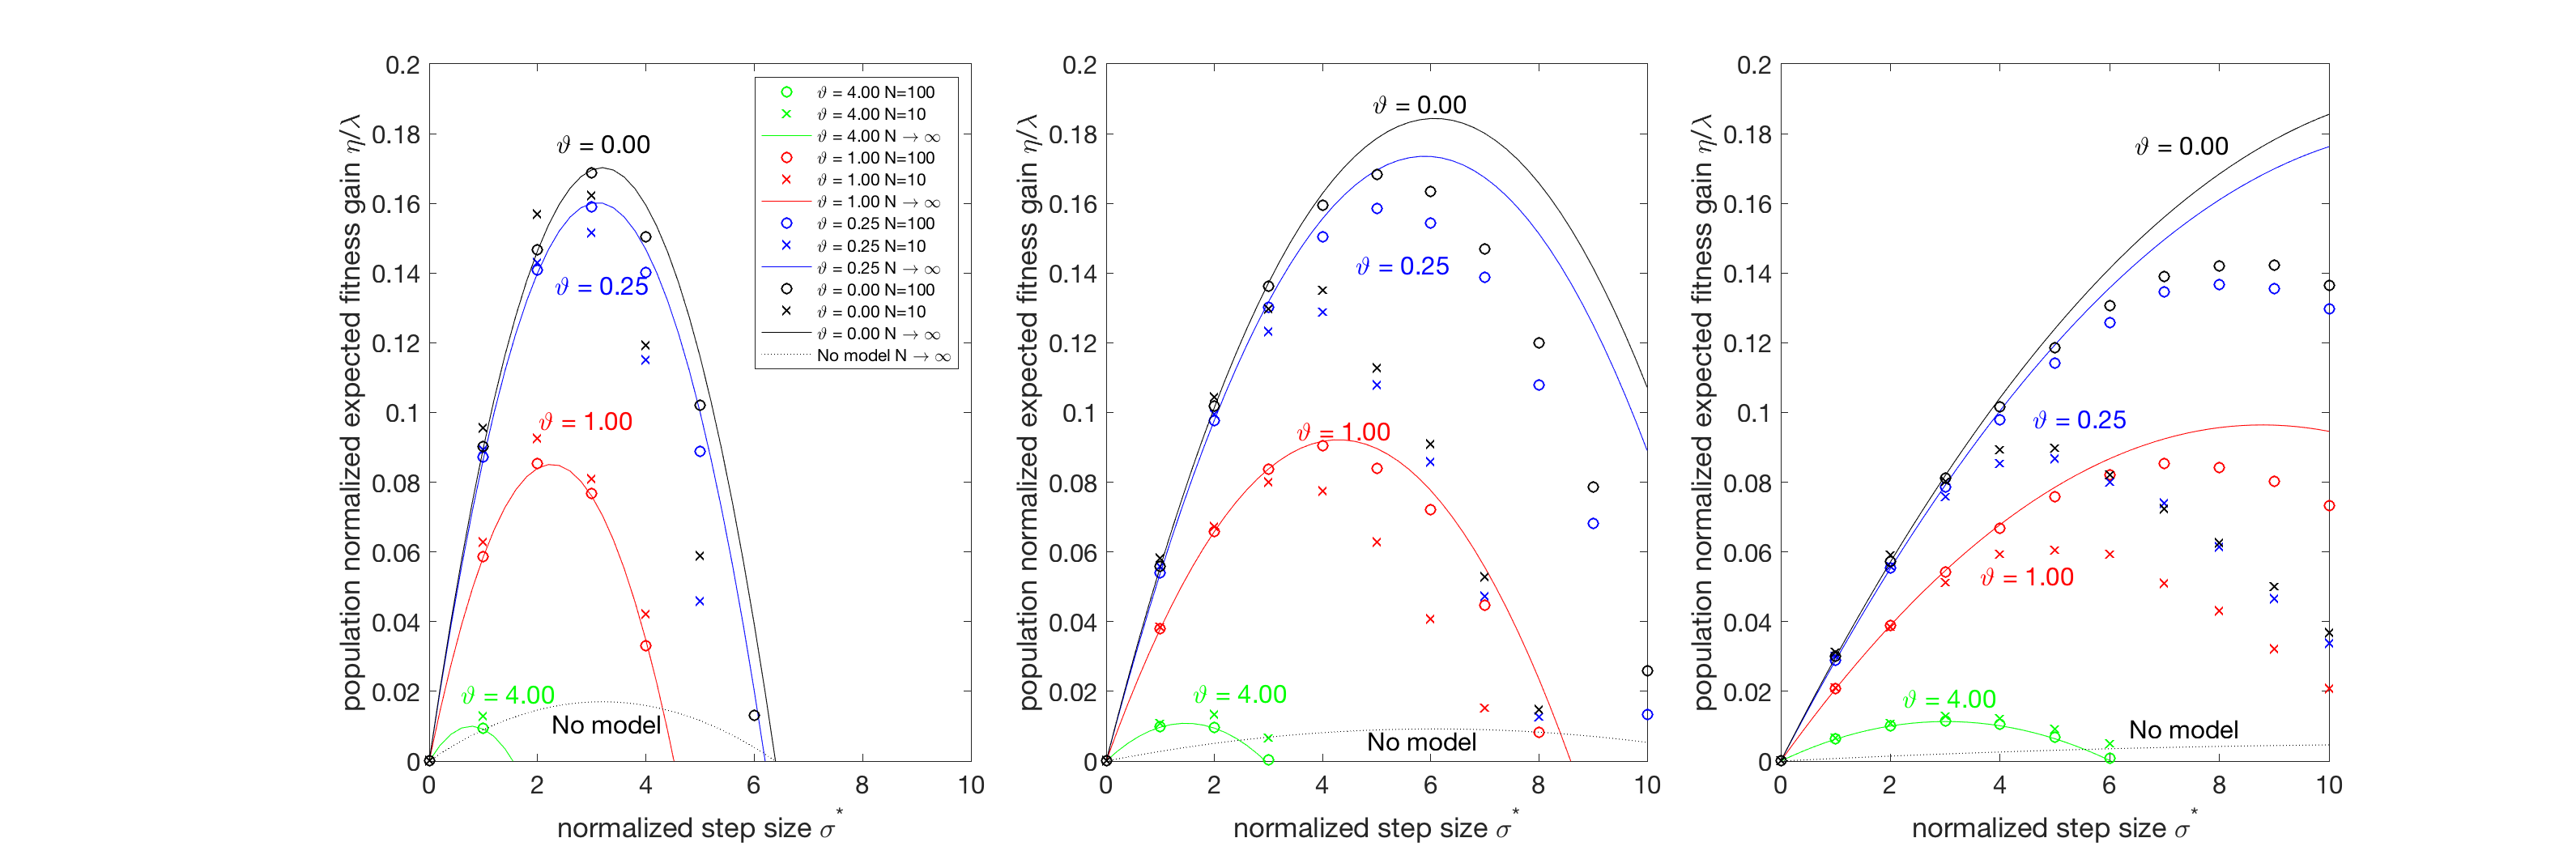
\includegraphics[height=2.1in, width=6.0in]{expectedFitGain_final_2}
\caption{The figures from left to right show the expected single step behaviour of the surrogate model assisted $(\mu/\mu,\lambda)$-ES with unbiased Gaussian distributed surrogate error for $\lambda=10,20,40\ (\mu = \lceil \lambda/4 \rceil)$ respectively. The solid lines are the results obtained analytically when $N \rightarrow \infty$; the dotted lines in the bottom of the figures show the relationship for corresponding $(\mu/\mu,\lambda)$-ES without surrogate model assistance (when $N\rightarrow \infty$); the dots represent the experimental results for $N=10$ (crosses) and $N=100$ (circles). 
}
\label{fig:expectedFitGain}
\end{figure*}
\end{center}

To obtain the opt. expected fitness gain $\eta_{opt}$ and its corresponding opt. normalized step size $\sigma^*_{opt}$ over a fixed noise-to-signal ratio $\vartheta$, by assuming independence of $\vartheta$ and $\sigma^*$, we take the derivative of equation (\ref{eqn:eta_surrogate}) over $\sigma^*$ and obtain
\begin{align}\label{eqn:opt_surrogate}
\sigma^*_{opt} &= \frac{ \mu c_{\mu / \mu, \lambda}}{\sqrt {1+ \vartheta^2}}\\
\eta_{opt} &= \frac{\sigma^*_{opt} c_{\mu / \mu, \lambda}}{\sqrt {1+ \vartheta^2}} - \frac{(\sigma^*_{opt})^2}{2 \mu} 
\end{align}

 For easy comparison, the expected fitness gain is normalized regarding the population size $\lambda$; the normalized fitness gains for all strategies are divided by their corresponding population size $\lambda$ (i.e., $\eta/\lambda$ is plotted against $\sigma^*$) in Fig. \ref{fig:expectedFitGain} . The population-normalized fitness gains against the normalized step size for the $(\mu/\mu,\lambda)$-ES with population size $\lambda=10,20,40$ and corresponding $\mu=3,5,10$ are plotted from left to right in Fig. \ref{fig:expectedFitGain}. The lines show the population-normalized results obtained (after normalization regarding population size $\lambda$) from Eqs. (\ref{eqn:c_mu_mu_lambda}), (\ref{eqn:eta_noise_sphere}), (\ref{eqn:eta_surrogate}), and Eqs. (4), (6), $\eta = E[\Delta]/p_{\text{eval}}$ (from the surrogate model assisted (1+1)-ES \cite{DBLP:conf/ppsn/KayhaniA18}). The dots represent the experimental results of unbiased Gaussian surrogate error for $N \in \{10,100 \}$ obtained by averaging 100 runs. 

% Copy from Arash's paper
% The results obtained for $N \rightarrow \infty$ are cases with a large normalized step size and very small noise-to-signal ratio. 

It can be inferred from Fig. \ref{fig:expectedFitGain} that, for a fixed population size, the expected fitness gain decreases as the noise-to-signal-ratio $\vartheta$ increases. When $\vartheta \rightarrow \infty$, the surrogate model becomes useless, and the strategy becomes a random search. For moderate noise-to-signal ratio $\vartheta$, the surrogate model assisted $(\mu/\mu,\lambda)$-ES can achieve much larger opt. expected fitness gain at a larger normalized step size compared with the surrogate model assisted (1+1)-ES \cite{DBLP:conf/ppsn/KayhaniA18}. When $\vartheta = 1$, the maximal expected fitness gain achievable for $(3/3,10)$-ES, $(5/5,20)$-ES, and $(10/10,40)$-ES are 0.8426, 1.841, and 3.856 with corresponding $\sigma^*=2.258,4.294$, and $8.769$ respectively; for surrogate model assisted (1+1)-ES, the maximal fitness gain is 0.548 achieved at $\sigma^* = 1.905$. As for $(\mu/\mu,\lambda)$-ES and (1+1)-ES both without model assistance, the maximal fitness gains are 0.202, 0.170, 0.184, and 0.193 achieved at $\sigma^*=1.224,3.200,6.080$, and $12.420$ for $(1+1)$-ES, $(3/3,10)$-ES, $(5/5,20)$-ES, and $(10/10,40)$-ES respectively. The value of maximal fitness achievable for $(\mu/\mu,\lambda)$-ES without surrogate model assistance grows as $\lambda$ increases and gradually approaches 0.202, which asymptotically equals to that of the $(1+1)$-ES \cite{Beyer:1995:TTE:1326683.1326688}. From the above analysis, surrogate assisted $(\mu/\mu,\lambda)$-ES does benefit from using a larger population, namely, the expected maximal fitness gain increased by a factor of $\lambda$ after the surrogate model is applied; and an observable improvement in opt. fitness gain achieved at a larger normalized step size compared with the surrogate model assisted (1+1)-ES. For $\vartheta=0$ (the surrogate model models the objective function exactly), from Eqn. (\ref{eqn:opt_surrogate}) we can obtain the maximal expected fitness gain for surrogate assisted $(\mu/\mu,\lambda)$-ES achieved at $\sigma^*_{opt} = \ \mu c_{\mu / \mu, \lambda}$ with value $\eta_{opt} =  \mu (c_{\mu / \mu, \lambda})^2/2$. Even if this indicates the potential benefit of using a growing population size, it is important to note the analytical result derived when $N \rightarrow \infty$ is an approximation for the finite-dimensional case. Fig. \ref{fig:opt_stepSize_fitGain} shows the relation of optimal expected fitness gain and the corresponding optimal normalized step size over noise-to-signal ratio derived analytically in the limit of $N \rightarrow \infty$ for $(\mu/\mu,\lambda)$-ES with $\lambda=10,20,40$ and (1+1)-ES, all including cases with and without surrogate model assistance. The optimal expected fitness gain is also measured experimentally for $n \in \{10,100 \}$. 
   
\begin{center}
\begin{figure*}
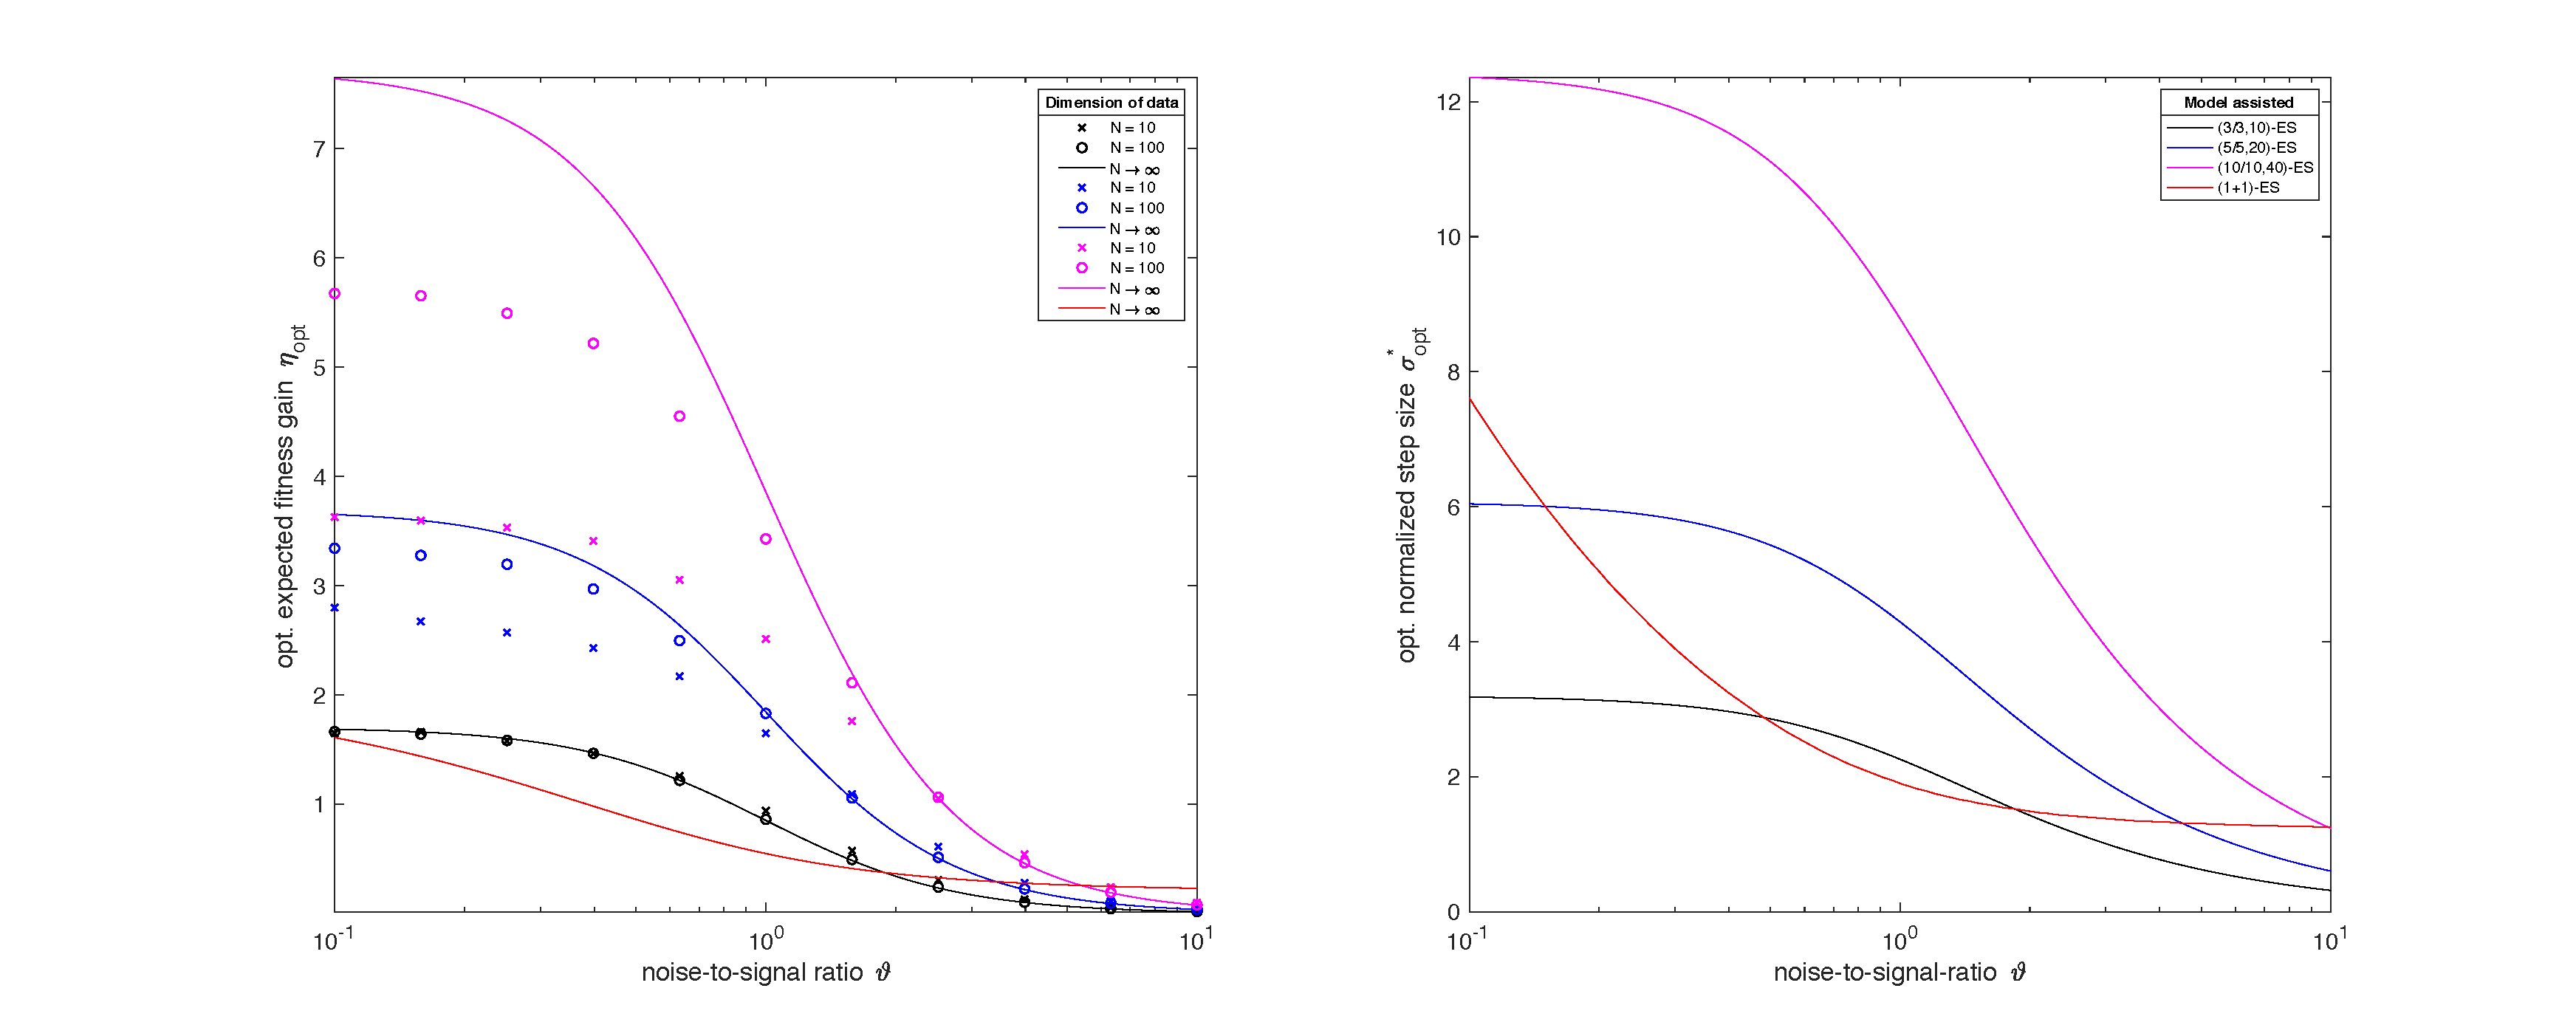
\includegraphics[height=2.4in, width=6in]{opt_stepSize_fitGain_final}
\caption{Opt. expected fitness gain and corresponding opt. normalized step size of the surrogate model assisted $(\mu/\mu,\lambda)$-ES and (1+1)-ES plotted against the noise-to-signal ratio. Colour black, blue, magenta and red represent the result for $(3/3,10)$-ES, $(5/5,20)$-ES, $(10/10,40)$-ES and (1+1)-ES respectively.The solid line represents the results obtained analytically when $N\rightarrow \infty$. The dots are the experimental result for N = 10 (crosses) and N = 100. The dotted lines show the optimal values for the $(3/3,10)$-ES, $(5/5,20)$-ES, $(10/10,40)$-ES and (1+1)-ES without surrogate model assistance. 
}
\label{fig:opt_stepSize_fitGain}
\end{figure*}
\end{center}


\begin{table*} 
\caption{Speed-ups for a small noise-to-signal ratio ($\vartheta=0.1$) observed in analysis}
\begin{tabular}{ l *{5}{D{.}{.}{5}} }
\toprule
\textbf{} & \multicolumn{5}{c}{\textbf{Different Evolution Strategy used for comparison}} \\
% To control the lines above different ES
\cmidrule(lr){2-5}
\textbf{speed-up} &  \multicolumn{1}{c}{(1+1)-ES} &  \multicolumn{1}{c}{$(3/3,10)$-ES} & \multicolumn{1}{c}{$(5/5,20)$-ES} & \multicolumn{1}{c}{$(10/10,40)$-ES}   \\
\midrule
\texttt{$\text{speed-up}_{\text{self}}(N=10)$} 	      & 4.1 &9.9  &15.2  &18.8     \\
\texttt{$\text{speed-up}_{\text{self}}(N=100)$}       & 6.8 &9.9  &18.1  &29.4   \\ 
\texttt{$\text{speed-up}_{\text{self}}(N \rightarrow \infty)$} & 8.0 &10.0  &20.0  &40.0     \\
\texttt{$\text{speed-up}_{\text{model}}(N=10)$}       &     &1.6  &3.0   &6.2  \\ 
\texttt{$\text{speed-up}_{\text{model}}(N=100)$}      &     &1.7  &3.3   &6.6  \\
\bottomrule             
\end{tabular}
\label{Tab:Test_result_analysis}
\end{table*}


\begin{table*} 
\caption{Speed-ups for moderate noise-to-signal ratio ($\vartheta=1$) observed in analysis}
\begin{tabular}{ l *{5}{D{.}{.}{5}} }
\toprule
\textbf{} & \multicolumn{5}{c}{\textbf{Different Evolution Strategy used for comparison}} \\
% To control the lines above different ES
\cmidrule(lr){2-5}
\textbf{speed-up} &  \multicolumn{1}{c}{(1+1)-ES} &  \multicolumn{1}{c}{$(3/3,10)$-ES} & \multicolumn{1}{c}{$(5/5,20)$-ES} & \multicolumn{1}{c}{$(10/10,40)$-ES}   \\
\midrule
\texttt{$\text{speed-up}_{\text{self}}(N=10)$} 	      & 2.7 &5.1  &9.0  &13.0     \\
\texttt{$\text{speed-up}_{\text{self}}(N=100)$}       & 2.7  &5.5  &9.9  &17.8   \\ 
\texttt{$\text{speed-up}_{\text{self}}(N \rightarrow \infty)$} & 2.9 &5.9  &10.0  &19.9     \\
\texttt{$\text{speed-up}_{\text{model}}(N=10)$}       &     &2.4  &3.7   &4.6  \\ 
\texttt{$\text{speed-up}_{\text{model}}(N=100)$}      &     &1.5  &2.7   &4.4  \\
\bottomrule             
\end{tabular}
\label{Tab:Test_result_analysis_eta_1}
\end{table*}

The speed-up is defined as the median number of objective function evaluations used to solve the test problems (when reaching the termination criteria) using one strategy divided by that of using the surrogate model assisted ES, both using the opt. normalized step size. For comparison purposes, we define two speed-ups, namely $\text{speed-up}_{\text{self}}$ and $\text{speed-up}_{\text{model}}$. $\text{speed-up}_{\text{self}}$ is defined as the number of objective function calls used for a surrogate model assisted ES divided by that of the ES without surrogate model assistance (specifically $(\mu/\mu,\lambda)$-ES if the ES is not specified); and $\text{speed-up}_{\text{model}}$ as the number of objective function calls needed for (1+1)-ES to solve the problem divided by that of $(\mu/\mu,\lambda)$-ES, both with surrogate model assistance. The results obtained for noise-to-signal $\vartheta =0.1$ and $1$ are shown in Table \ref{Tab:Test_result_analysis} anf Table \ref{Tab:Test_result_analysis_eta_1}.
% Not a problem
%$\color{red}{\text{wonder if there is need to describe the results in the table again (as is done in the following two paragraphs)}}$  




For a finite-dimension e.g. $N=10$, the $\text{speed-up}_{\text{self}}$ achieved for small noise-to-signal ratio ($\vartheta=0.1$) appears to be around nine and ten for a population size $\lambda=10$, fifteen and sixteen for $\lambda = 20$, eighteen and nineteen for $\lambda=40$; whereas for (1+1)-ES, the $\text{speed-up}_{\text{self}}$ tops out between four and five. When $N=100$, the $\text{speed-up}_{\text{self}}$ for small noise-to-signal ratio are between nine and ten, eighteen and nineteen, and twenty-nine and thirty for $(3/3,10)$-ES, $(5/5,20)$-ES, and $(5/5,40)$-ES respectively; as for (1+1)-ES, the $\text{speed-up}_{\text{self}}$ with a small noise-to-signal ratio is between six and seven when $N=100$. The $\text{speed-up}_{\text{self}}$ (for $(\mu/\mu,\lambda)$-ES) mounts with a growing population size $\lambda$, but it is worth noting that $\text{speed-up}_{\text{self}} \overset{N \rightarrow \infty}{\rightarrow} \lambda$, and the gap in $\text{speed-up}_{\text{self}}$ between a finite dimension (fixed) and infinite dimension increases as $\lambda$ grows (e.g., compared with $N\rightarrow \infty$, the $\text{speed-up}_{\text{self}}$ achieved when $N=10$ decreases 1\%, 24\%, and 53\% for $\lambda=10,20$, and $40$ respectively).  
%\mid_{N=10}$ of $\text{speed-up}_{\text{self}}$ (between experimental results of $N=10,100$ using same population size) decrease as $\lambda$ grows.$\color{red}{\text{wonder if it is worthing comparing the speed-up in a finite dimension and infinite case.}}$  

When comparing (1+1)-ES and $(\mu/\mu,\lambda)$-ES both with surrogate model assistance, $\text{speed-up}_{\text{model}}$ for $(3/3,10)$-ES, $(5/5,20)$-ES, and $(5/5,40)$-ES when $N=10$ are between two and three, three and four, four and five respectively; whereas $N=100$, the $\text{speed-up}_{\text{model}}$ decrease to a value between one and two, two and three, and four to five respective for $\lambda=10,20,$ and $40$. From the observed result, the speed-up for surrogate model assisted $(\mu/\mu,\lambda)$-ES is significant over both the surrogate model assisted (1+1)-ES and $(\mu/\mu,\lambda)$-ES without model assistance. It seems that the expected fitness gain for the surrogate assisted $(\mu/\mu,\lambda)$-ES will increase in line with population size $\lambda$, especially with a large dimensionality. Besides, the shrinking gap in $\text{speed-up}_{\text{model}}$ between different finite dimension over a growing population (i.e., the $\text{speed-up}_{\text{model}}$ for $N=100$ approaches that of $N=10$ as $\lambda$ grows) also suggests using a larger $\lambda$ for potential stable $\text{speed-up}_{\text{model}}$ compared with the surrogate assisted (1+1)-ES. Although the analytical results obtained for $N\rightarrow \infty$ are approximations in the finite-dimension and can be inaccurate but it gives an implication for using larger $\lambda$ for potential larger fitness gain.

% "Gives an implication" is vague enough not to get you into trouble here.  It sounds a little unusual though.
% $\color{red}{\text{wonder if gives too many implications and can be a trouble in terms of burden of proof.}}$  









%%%%%%%%%%%%%%%%%%%%%%%%%%%%%%%%%%%%%%%%%%%%%%%%%%%%%%%%%%%%%%%%%%%%%%%%%%%%%%%%%%%%%%%%%%%%
%%%%%%%%%%%%%%%%%%%%%%%%%%%%%%%%%%%%%%%%%%%%%%%%%%%%%%%%%%%%%%%%%%%%%%%%%%%%%%%%%%%%%%%%%%%%
\section{Step size adaptation}\label{sec:step_size_adaptation}

\subsection{Cumulative step size adaptation}

\begin{algorithm}
\caption{Surrogate Model Assisted $(\mu/\mu,\lambda)$-ES (GP-$(\mu/\mu,\lambda)$-ES)}
\label{alg:GP-mml-es}
\begin{algorithmic}[1]
\STATE $c \leftarrow  \frac{\mu +2}{N+\mu+5}$ 
\STATE $d \leftarrow 1 + 2 \text{max}(0, \sqrt{\frac{\mu - 1}{N+1} } - 1 ) + c$
\STATE $E \left\lVert  \mathcal{N}(0,I) \right\rVert \approx \sqrt{N}(1 - \frac{1}{4N} + \frac{1}{21N^2})$
\STATE $s^{(0)} \leftarrow 0$

\WHILE{not terminate()} 
	\FOR{$i=1,2,...,\lambda$}
		\STATE Generate standard normally distributed $z_i^{(g)} \in \mathbb{R}^N $
		% \STATE $y_i^{(g)} \leftarrow x_{\text{centroid}}^{(g)} + \sigma^{(g)} z_i$
		\STATE Evaluate $x_{\text{centroid}}^{(g)} + \sigma^{(g)} z_i^{(g)}$ using the surrogate model, yielding $f_{\epsilon}(x_{\text{centroid}}^{(g)} + \sigma^{(g)} z_i)$
	\ENDFOR
	% \STATE $fY_{\epsilon}^{(g)} \leftarrow \{f_{\epsilon}(x_{\text{centroid}}^{(g)} + \sigma^{(g)} z_i^{(g)}): i=1,2,...,\lambda\}$
	% \STATE $z_{\text{step}}^{(g)} \leftarrow \frac{1}{\mu} \sum_{i=1}^{\mu} z_{i;\lambda}^{(g)}$, where $z_{i;\lambda}^{(g)} \in$ select\_best $(\mu,\{ \},fY_{\epsilon}^{(g)})$
	% \STATE $X^{(g+1)} \leftarrow  select\_best (\mu,Y^{(g)},fY_{\epsilon}^{(g)})$
	\STATE $z_{\text{step}}^{(g)} \leftarrow \frac{1}{\mu}\sum_{i=1}^{\mu} z_{i;\lambda}^{(g)}$
	\STATE $x_{\text{centroid}}^{(g+1)} \leftarrow  x_{\text{centroid}}^{(g)} + \sigma^{(g)} z_{\text{step}}^{(g)}$ 
	\STATE Evaluate $x_{\text{centroid}}^{(g+1)}$ using true objective function, yieding $f(x_{\text{centroid}}^{(g+1)})$
	\STATE Update surrogate model by adding $(x_{\text{centroid}}^{(g+1)},f(x_{\text{centroid}}^{(g+1)}))$
	\STATE $s^{(g)} \leftarrow (1-c)s + \sqrt{ c(2-c) \mu} z_{\text{step}}^{(g)}$
	\STATE $\sigma^{(g+1)} \leftarrow \sigma^{(g)}  \text{exp} \left(\frac{c}{d} \frac{\left\lVert s^{(g)} \right\rVert} { E \left\lVert \mathcal{N}(0,I) \right\rVert} -1 \right )$
	\STATE $g \leftarrow g + 1$
\ENDWHILE

\end{algorithmic}
\end{algorithm}

% \begin{algorithm}
% \caption{Surrogate Model Assisted $(\mu/\mu,\lambda)$-ES}
% \label{alg:mml-es}
% \begin{algorithmic}[1]
% \STATE $c \leftarrow  \frac{\mu +2}{n+\mu+5}$ 
% \STATE $d \leftarrow 1 + 2 \text{max}(0, \sqrt{\frac{\mu - 1}{n+1} } - 1 ) + c$
% \STATE $s^{(0)} \leftarrow 0$

% \WHILE{not terminate()} 
% 	\FOR{$i=1,2,...,\lambda$}
% 		\STATE Generate standard normally distributed $z_i \in \mathbb{R}^N $
% 		\STATE $y_i^{(g)} \leftarrow x_{\text{centroid}}^{(g)} + \sigma^{(g)} z_i$
% 		\STATE Evaluate $y_i^{(g)}$ using the surrogate model, yieding $f_{\epsilon}(y_i^{(g)})$
% 	\ENDFOR
% 	\STATE $Y^{(g)} \leftarrow \{y_i^{(g)}: i=1,2,...,\lambda\}$
% 	\STATE $fY_{\epsilon}^{(g)} \leftarrow \{f_{\epsilon}(y_i^{(g)}): i=1,2,...,\lambda\}$
% 	% \STATE $z_{\text{step}}^{(g)} \leftarrow \frac{1}{\mu} \sum_{i=1}^{\mu} z_{i;\lambda}^{(g)}$, where $z_{i;\lambda}^{(g)} \in$ select\_best $(\mu,\{ \},fY_{\epsilon}^{(g)})$
% 	\STATE $X^{(g+1)} \leftarrow  select\_best (\mu,Y^{(g)},fY_{\epsilon}^{(g)})$
% 	\STATE $x_{\text{centroid}}^{(g+1)} \leftarrow  recombine(X^{(g+1)})$ 
% 	\STATE Evaluate $x_{\text{centroid}}^{(g+1)}$ using true objective function, yieding $f(x_{\text{centroid}}^{(g+1)})$
% 	\STATE Update surrogate modle by adding $(x_{\text{centroid}}^{(g+1)},f(x_{\text{centroid}}^{(g+1)}))$
% 	\STATE $s^{(g)} \leftarrow (1-c)s + \sqrt{ c(2-c) \mu} z_{\text{step}}$
% 	\STATE $\sigma^{(g+1)} \leftarrow \sigma^{(g)}  \text{exp} \left(\frac{c}{d} \frac{\left\lVert X \right\rVert} { E \left\lVert N(0,I) \right\rVert} -1 \right )$
		

% \ENDWHILE

% \end{algorithmic}
% \end{algorithm}

Even though the analysis in Section \ref{sec:analysis} suggests a potential better performance for the surrogate-assisted $(\mu/\mu,\lambda)$-ES. There is no guarantee that the step size of the strategy can be properly adapted, and further the analysis is very inaccurate in terms of finite dimension. In this section we experiment the surrogate model assisted $(\mu/\mu,\lambda)$-ES using the CSA described in Section \ref{sssec:def_ES} and \ref{sssec:step_size_adaptation}, and exploit the potential insight it may offer. The strategy is evaluated using a Gaussian Process surrogate model in place of the simple model described in Section \ref{sec:analysis}; one single iteration of the surrogate model assisted $(\mu/\mu,\lambda)$-ES using CSA (referred to as GP-$(\mu/\mu,\lambda)$-ES) is shown in Alg. \ref{alg:GP-mml-es} where $z_{i;\lambda}^{(g)}$ denotes the ith best mutation ranked according to the fitness of the corresponding offspring estimated by the surrogate model that has $f_{\epsilon}(x_{\text{centroid}}^{(g)} + \sigma^{(g)} z_{i;\lambda}^{(g)})<f_{\epsilon}(x_{\text{centroid}}^{(g)} + \sigma^{(g)} z_{j;\lambda}^{(g)}),1 \leq i < j \leq \lambda$. 

Five ten-dimensional test problems are used to test if the step size of the strategy has been appropriately adapted, namely sphere functions $f(x) = (x^Tx)^{\alpha/2}$ for $\alpha = \{1,2,3 \}$, referred to as linear, quadratic, and cubic spheres; $f(x) = \sum_{i=1}^N(\sum_{j=1}^i x_j)^2$ (i.e., a convex quadratic function with condition number of the Hessian approximately equal to 175.1) referred to as Schwefel's Problem 1.2 \cite{Schwefel:1981:NOC:539468}); and quartic function \cite{DBLP:conf/ppsn/KayhaniA18} defined as $f(x) = \sum_{i=1}^{N-1} \left[ \beta(x_{i+1} -x_i^2)^2 + (1-x_i)^2 \right]$ where $\beta = 1$. For $\beta=1000$, the quartic function becomes the Rosenbrock function with the condition number of the Hessian at the optimizer exceeds 3,500, making it very hard to find the global optimum without adapting the shape of the mutation distribution. So we use the quartic function with $\beta=1$ in the context where the corresponding condition number of the Hessian at the optimizer equals to 49.0. The values of global optima for all test function are zero. For each test problem, 100 runs are conducted for (1+1)-ES, (3/3,10)-ES, (5/5,20)-ES, (10/10,40)-ES both with and without surrogate model assistance. 

% surrogate assisted $(\mu/\mu,\lambda)$-ES using $\lambda=10,20,40$ and corresponding $\mu = \lceil \lambda / 4 \rceil$ both with and without surrogate model assistance where a parental population size $\lambda=10,20,40$ with  are used. $(1+1)$-ES and 

For surrogate model, we use Gaussian process with squared exponential kernel and the length scale parameter in the kernel is set proportional to both the step size of the ES and the square root of data dimension $N$. For simplicity, the length scale is set to $8 \sigma \sqrt{N}$ as is used in the surrogate assisted (1+1)-ES \cite{DBLP:conf/ppsn/KayhaniA18}. In our experience, using a smaller or larger value by a factor of two i.e., $2,4$ and $16,32$ does not give a significant improvement, so we stick to $8$ in the context.

\begin{table*} 
\caption{Median test results for $(\mu/\mu,\lambda)$-ES without surrogate model assistance.}
\begin{tabular}{ l *{4}{D{.}{.}{4}} }
\toprule
\textbf{} & \multicolumn{4}{c}{\textbf{Median number of objective function calls  }} \\
\cmidrule(lr){2-5}
\textbf{Test functions} &  \multicolumn{1}{c}{$(3/3,10)$-ES} & \multicolumn{1}{c}{$(5/5,20)$-ES} & \multicolumn{1}{c}{$(10/10,40)$-ES}  \\
\midrule
\texttt{linear sphere} 	      &3300  &4809  &8405      \\
\texttt{quadratic sphere}     &1694  &2436  &4182   \\ 
\texttt{cubic sphere}         &1166  &1659  &2788    \\ 
\texttt{Schwefel' s function}&6259 & 8064 &13325 \\
\texttt{quartic function}     &6600 &8442 &14637   \\ 
\bottomrule             
\end{tabular}
\label{Tab:Test_result_noGP_mml}
\end{table*}


\begin{table*} 
\caption{Median test results and speed-ups of GP-$(\mu/\mu,\lambda)$-ES.}
\begin{tabular}{ l *{5}{D{.}{.}{6}} }
\toprule
\textbf{} & \multicolumn{5}{c}{\textbf{Median number of objective function calls ($\text{speed-up}_{\text{self}},\text{speed-up}_{\text{model}}$) }} \\
\cmidrule(lr){2-6}
\textbf{Test functions} & \multicolumn{1}{c}{$(1+1)$-ES} & \multicolumn{1}{c}{$(3/3,10)$-ES} & \multicolumn{1}{c}{$(5/5,20)$-ES} & \multicolumn{1}{c}{$(10/10,40)$-ES}  \\
\midrule
\texttt{linear sphere} 	      &502  &756(4.4,0.66)  &696(6.9,0.72)  &761(11.0,0.66)      \\
\texttt{quadratic sphere}     &214  &309(5.5,0.69)  &245(9.9,0.87)  &231(18.1,0.93)    \\ 
\texttt{cubic sphere}         &205  &273(4.3,0.75)  &249(6.7,0.82)  &253(6.7,0.81)    \\ 
\texttt{Schwefel' s function}&1503  & 2278(2.7,0.66) & +\infty(/) & +\infty(/)\\
\texttt{quartic function}     &1265 &1000(6.6,1.3) &746(11.3,1.7) &667(21.9,1.9)    \\ 
\bottomrule             
\end{tabular}
\label{Tab:Test_result_GP-mml-ES}
\end{table*}

\begin{center}
\begin{figure*}
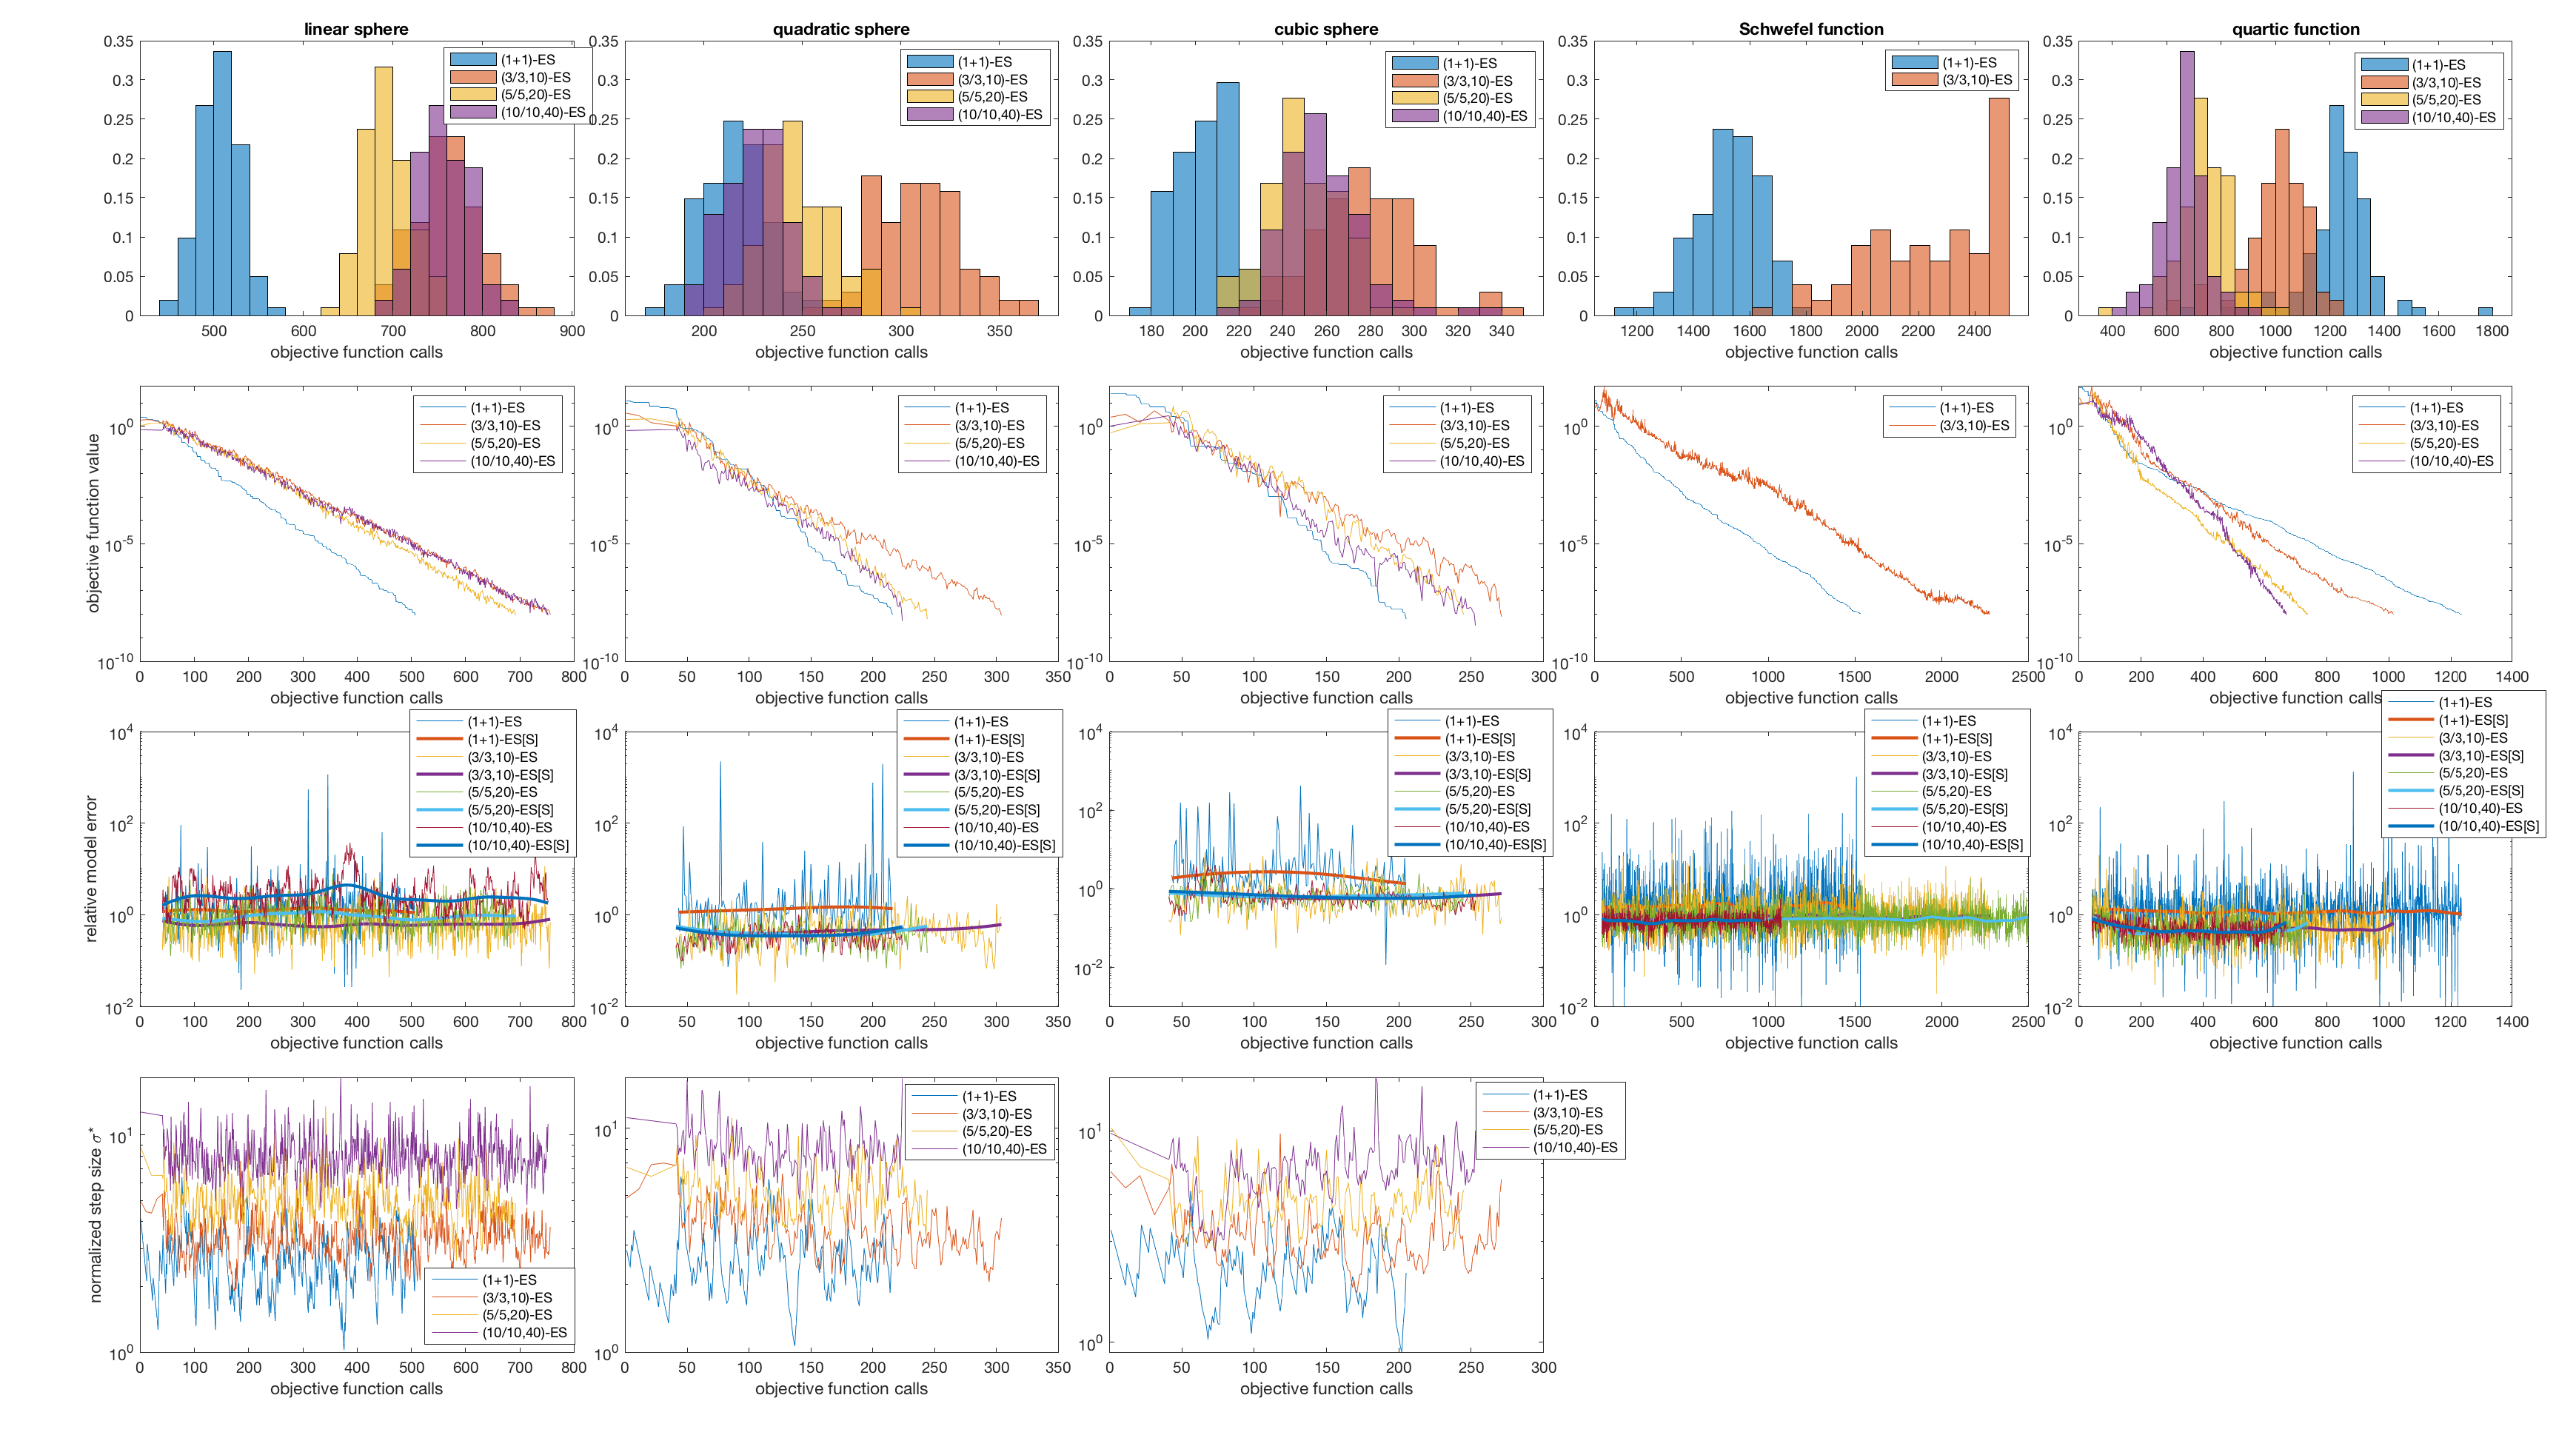
\includegraphics[height=4.3in, width=6.1in]{merged_plot_NO_emergency_v4_final}
\caption
{Results for GP-$(\mu/\mu,\lambda)$-ES (with GP and CSA applied). Top row: Histograms showing the number of objective function calls needed to solve the five test problems. Second row: Convergence graphs observed in median runs. Third row: Relative model error obtained in median runs ([S] denotes the smoothed relative model error). Last row: Normalized step size measured in median runs for sphere functions.
} 
\label{fig:merged_plot_GP-mml-ES}
\end{figure*}
\end{center}


The Gaussian process kernel is constructed using a training size of 40. The training set consists of the 40 most recent candidate solutions evaluated, so that the surrogate model approximates the local landscape of the objective function. All runs are initialized with starting point sampled from a Gaussian distribution with zero mean and unit covariance matrix and initial step size $\sigma_0=1$. The termination criteria is defined as one solution achieves objective function value below $10^{-8}$.

Histograms showing the number of objective function calls needed to solve the test problems within the required accuracy are represented in the first row of Fig. \ref{fig:merged_plot_GP-mml-ES}, the median number of objective function calls required to solve each test problem for $(\mu/\mu,\lambda)$-ES without and with surrogate model assistance (the step size of both are adapted using CSA) is shown in Table \ref{Tab:Test_result_noGP_mml} and Table \ref{Tab:Test_result_GP-mml-ES} respectively; the result for surrogate assisted (1+1)-ES \cite{DBLP:conf/ppsn/KayhaniA18} is also included in Table \ref{Tab:Test_result_GP-mml-ES} for comparison. 


The two speed-ups $\text{speed-up}_{\text{self}}$ and $\text{speed-up}_{\text{model}}$ defined in Section \ref{sec:analysis} are used.  The $\text{speed-up}_{\text{self}}$ on quadratic sphere for GP-$(\mu/\mu,\lambda)$-ES with $\lambda=10,20,40$($\mu = \lceil \lambda/4 \rceil $) are between five and six, nine and ten, eighteen and nineteen respectively; whereas the corresponding expected results obtained in Analysis are between nine and ten, fifteen and sixteen, eighteen and nineteen respectively. There is a gap between the expected performance (in Section \ref{sec:analysis}) and the experimental results (after the GP surrogate model and CSA is in place) for GP-$(\mu/\mu,\lambda)$-ES. But the difference between expected values and observed values obtained through experiments seems to shrink as the population size $\lambda$ grows. In terms of $\text{speed-up}_{\text{model}}$, the achieved values for GP-$(\mu/\mu,\lambda)$-ES on quadratic sphere are about 0.7, 0.9, and 0.9 for $\lambda=10,20,40$ respectively, which is far from the expected maximal value of roughly 2.4, 3.7, and 4.6 obtained in \ref{Tab:Test_result_analysis_eta_1} when noise-to-signal ratio $\eta=1$. There is about a factor of four in terms of the expected maximal $\text{speed-up}_{\text{model}}$ and the results obtained in table \ref{Tab:Test_result_GP-mml-ES}. The $\text{speed-up}_{\text{self}}$ observed for sphere functions are between four and five for GP-$(\mu/\mu,\lambda)$-ES with $\lambda=10$, six and ten for GP-$(\mu/\mu,\lambda)$-ES with $\lambda=20$, and six to nineteen for GP-$(\mu/\mu,\lambda)$-ES with $\lambda=40$. It is interesting that only GP-$(\mu/\mu,\lambda)$-ES using $\lambda=10$ solves the 10-dimensional Schwefel's function, the increasing population does not give an advantage for solving the problem compared with the (1+1)-ES with surrogate model assistance, but rather a trend for divergence. Overall, the performance of GP-$(\mu/\mu,\lambda)$-ES does not match that of the surrogate model assisted (1+1)-ES, specifically, $\text{speed-up}_{\text{model}}<1$ for all test functions except quartic function where the observed $\text{speed-up}_{\text{model}}$ are about 1.3, 1.7, and 1.9 for population size $\lambda=10,20,40$ respectively. It seems a growing population can possibly bring larger $\text{speed-up}_{\text{model}}$ for quadric sphere and quartic function, meanwhile it appears contrary to the other three test functions, especially the Schwefel's function. The $\text{speed-up}_{\text{self}}$ observed in linear and cubic sphere is lower than that in quadratic sphere, indicating a potential less accurate Gaussian process based surrogate model in the two sphere functions mentioned compared with the latter. 


% % Similarly, the $\text{speed-up}_{\text{self}}$s for surrogate assisted $(5/5,20)$-ES on sphere functions are between six and ten, while the results in Analysis are between fifteen and twenty; when $\lambda=40$ $\text{speed-up}_{\text{self}}$s range from six to eighteen for sphere functions, whereas the analytical result gives eighteen to forty.   

% Despite achieving a speed up between 1.2 and 1.9 for quartic function, the surrogate assisted $(\mu/\mu,\lambda)$-ES performs worse on sphere functions and even does not converge in Schwefel' s function with a large population $\lambda\geq20$. There is a trend in quadratic sphere and quartic function that the performance improves with a growing parental population while on cubic sphere, the performance is approximately the same when $n\geq 20$. When it comes to linear sphere, the number of objective function evaluations needed to solve the problem even increases after $\lambda>20$. 


The second row of Fig. \ref{fig:merged_plot_GP-mml-ES} shows the convergence graphs observed in median runs. Linear convergence are achieved for all but the Schwefel's function, specifically the using GP-$(\mu/\mu,\lambda)$-ES with $\lambda=20,40$. Interestingly, using a larger population on Schwefel's function does not help achieve faster convergence compared to (1+1)-ES, but instead, slows the  rate of convergence, and finally makes the strategy diverge. Relative model error for the median runs is shown in the third row of the figure. The relative model error in generation $(g)$ is defined as 
\begin{align}
\begin{cases}
\frac{\|f(y^{(g)})-f_{\epsilon}(y^{(g)}) \|}{\|f(y)-f_(x) \|},\text{for surrogate model assisted (1+1)-ES} \\
\sqrt{\frac{ var(fY^{(g)}-fY_{\epsilon}^{(g)})}{var(fY^{(g)}-fX^{(g)})}},\text{for surrogate model assisted }(\mu/\mu,\lambda)\text{-ES},
\end{cases}
\end{align}
where $x^{(g)}$ and $y^{(g)}$ are the parent and offspring in generation $(g)$ for surrogate model assisted (1+1)-ES from Kayhani and Arnold \cite{DBLP:conf/ppsn/KayhaniA18}; $fY^{(g)}- fX^{(g)}= \{ f(x_{\text{centroid}}^{(g)} + \sigma^{(g)} z_{\text{step}}^{(g)}) - f(x_{\text{centroid}}^{(g)}): 1 \leq i \leq \lambda \}$, $fY^{(g)}- fY_{\epsilon}^{(g)} = \{ f(x_{\text{centroid}}^{(g)} + \sigma^{(g)} z_{\text{step}}^{(g)}) - f_\epsilon (x_{\text{centroid}}^{(g)} + \sigma^{(g)} z_{\text{step}}^{(g)}) : 1 \leq i \leq \lambda \}$, and $var(fY^{(g)}- fY_{\epsilon}^{(g)})$ returns the variance of the $\lambda$ differences between the true and estimated objective function values for the offspring generated in generation $(g)$, and by taking square root over the division of two variances we can obtain the standard deviation similar to the case of surrogate model assisted (1+1)-ES. For easy comparison, the relative model error is smoothed logarithmically by convolution with a Gaussian kernel with window size 40 that is represented as the bold line in the centre of the plots (denoted [S] in the Fig.), interpreted as the a relative constant noise-to-signal ratio. The relative model error for all surrogate assisted ES in observed is approximately 1; but we notice the relative model error for GP-$(\mu/\mu,\lambda)$-ES is much smaller than that of the surrogate assisted (1+1)-ES, so is the variance of the relative model error. This is possibly the benefit of using a large population size. In linear sphere, the relative model error obtained by using GP-$(\mu/\mu,\lambda)$-ES with $\lambda=40$ is significantly higher compared with the rest strategies, which may explain the decline in $\text{speed-up}_{\text{model}}$ from 0.72 to 0.66 after $\lambda$ increased from 20 to 40. In the other problems, the relative model error for GP-$(\mu/\mu,\lambda)$-ES with different $\lambda$ seem to stay at the same level. In the quadratic sphere, the relative constant noise-to-signal ratio is approximately 0.7 for GP-$(\mu/\mu,\lambda)$-ES with different $\lambda$; and according to Fig. \ref{fig:opt_stepSize_fitGain}, when $\vartheta=0.7$, the opt. step size are between two and three, four and five, ten and eleven for $\lambda=10,20,40$ respectively. The corresponding expected $\text{speed-up}_{\text{model}}$ for $\lambda=10,20,40$ obtained by using the opt. expected fitness gain from Fig. \ref{fig:opt_stepSize_fitGain} when $\vartheta=0.7$ are about 1.7, 3.1, and 4.3 for $\lambda=10,20,40$ respectively. The bottom row in Fig. \ref{fig:merged_plot_GP-mml-ES} shows the normalized step size over the number of objective function calls observed in the median runs in the three sphere functions tested. The GP-$(\mu/\mu,\lambda)$-ES achieves a larger normalized step size $\sigma^*$ compared to the surrogate model assisted (1+1)-ES with $\sigma^*$ growing in line with $\lambda$, which coincides with our knowledge that using a larger population size in $(\mu/\mu,\lambda)$-ES can give a larger step size i.e., in the extreme case when $\lambda \rightarrow \infty $, we obtain the gradient at the current point (parent $x$). Given the relative constant noise-to-signal is 0.7 (i.e., $\vartheta=0.7$) for quadratic sphere, we can obtain the opt. expected normalized step size $\sigma^*$ from Fig. \ref{fig:opt_stepSize_fitGain} and compare that with the experimental result obtained in the bottom row of Fig. \ref{fig:merged_plot_GP-mml-ES}. The obtained $\sigma^*$ in experiment for each GP-$(\mu/\mu,\lambda)$-ES with different $\lambda$ is very close to that of the analytical result shown in Fig. \ref{fig:opt_stepSize_fitGain}, where the former ranges from two to four, four to six, nine to eleven for $\lambda=10,20,40$ respectively, and the latter has discussed above. The results indicates that the step size of the GP-$(\mu/\mu,\lambda)$-ES is appropriately adapted by CSA. 


% and according to the analysis in Section 3 should give a much larger speed up especially given a larger population. This may give indication that the step size is not appropriately adapted. The bottom row shows the normalized step size $\sigma^* = N \sigma/R$ for three sphere functions, where $N$,$R$ are the dimension of the data and distance to optimal respectively is the dimension. It coincides with the knowledge that using a population in offspring generation is possible for larger step size but the potential improvement is still yet clear. 


\begin{center}
\begin{figure*}
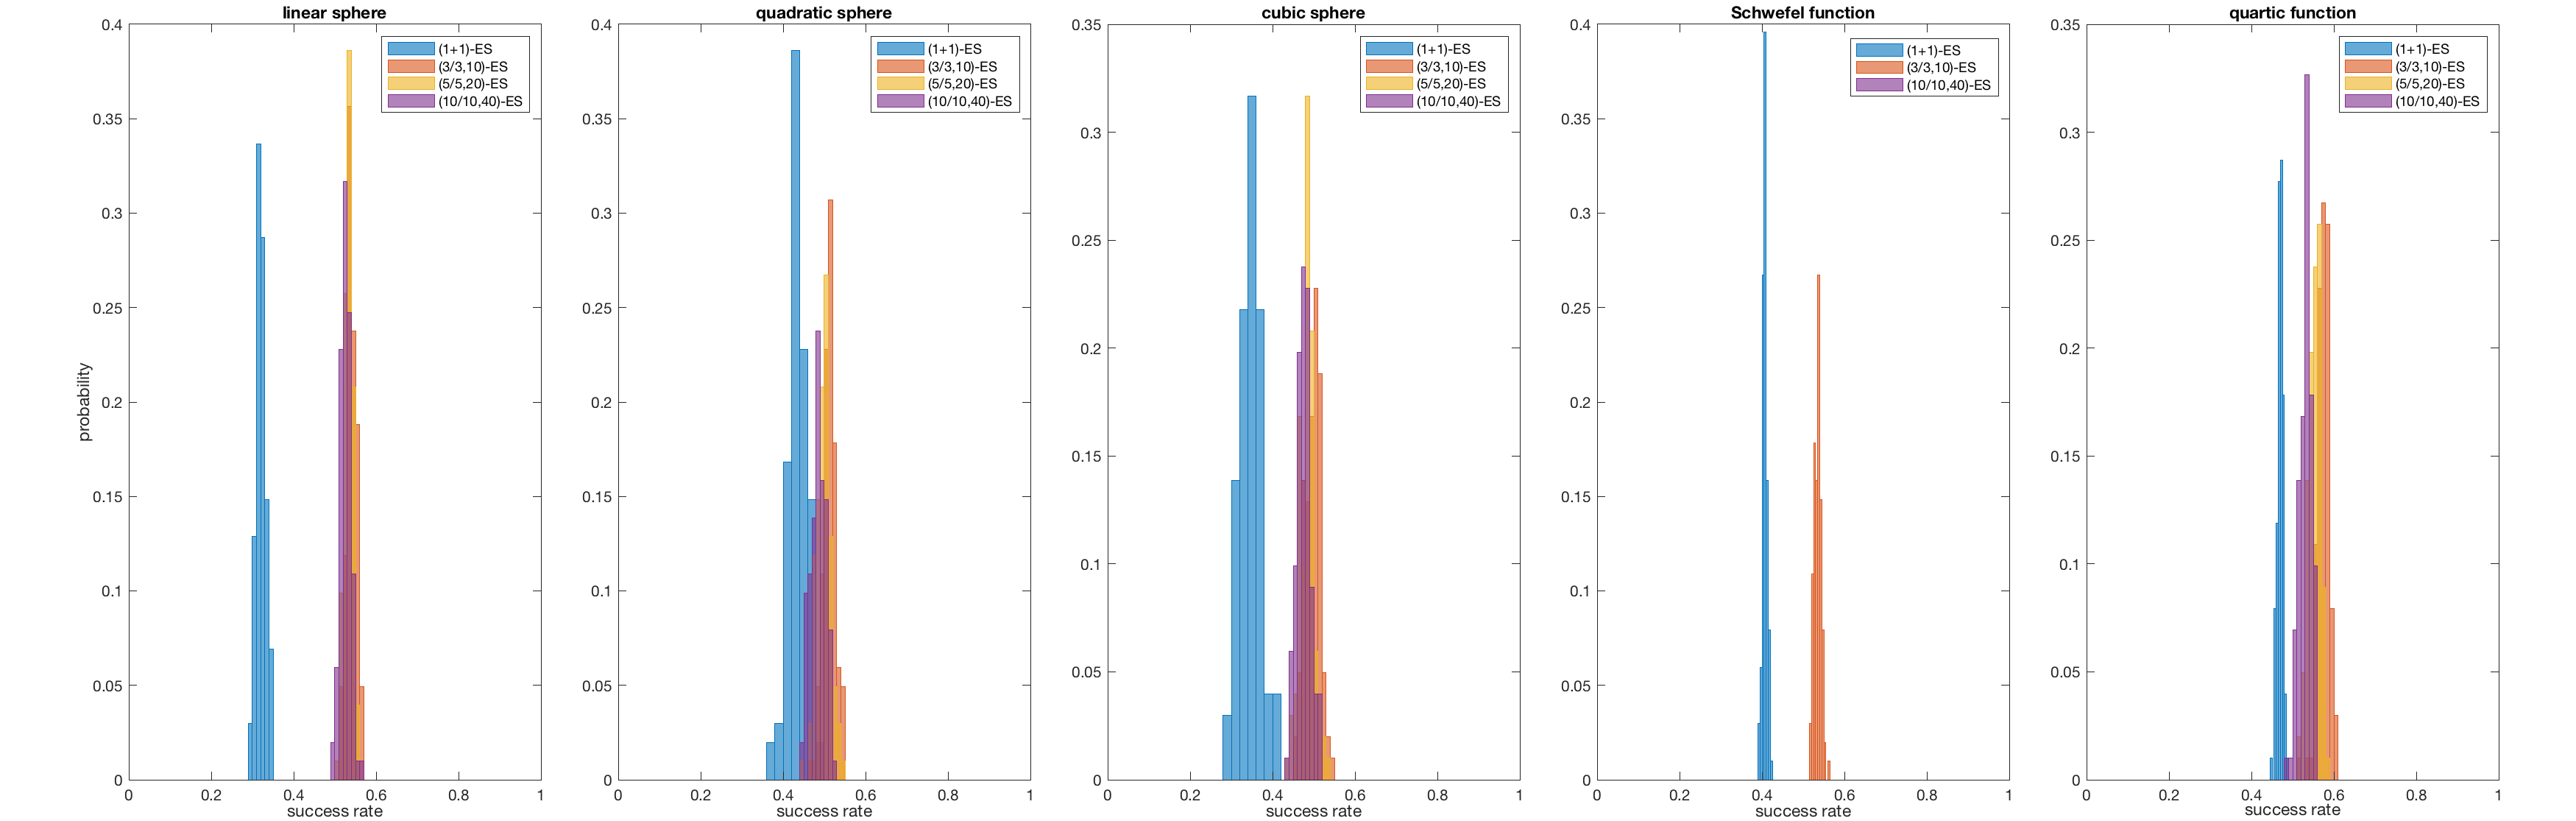
\includegraphics[height=1.2in, width=6in]{success_NO_emergency_v3_final.pdf}
\caption{Histograms of the success rate (proportion of good steps in a single run) for each test function using (1+1)-ES and GP-$(\mu/\mu,\lambda)$-ES with $\lambda=10,20,40$. 
}
\label{fig:success_plot_GP-mml-ES}


\end{figure*}
\end{center}


% Expected 		 1.7,3.1,4.3	  
% experimental   0.69,0.87,0.93

Despite the potentially well-adapted step size, there is a big gap between the expected $\text{speed-up}_{\text{model}}$ discussed above and the experimental result illustrated in Table \ref{Tab:Test_result_GP-mml-ES}. The reasons behind the resulting experimental results are not yet clear. Assuming the step size is well-adapted, the natural question to ask is what is the quality of the direction ($z_{\text{step}}$) used. If the resulting direction is poor (i.e., taking the direction cannot improve the fitness), the individual cannot gain any fitness even with an optimally adapted step size. On the other hand, taking a good step with a properly adapted step size can help generate better offspring (offspring with larger fitness gain compared with its parent). We further plot the histogram of success rate (the proportion of a good step in each run) for all test problems in Fig. \ref{fig:success_plot_GP-mml-ES} by replicating 100 runs for each test problems. Overall, the success rates for GP-$(\mu/\mu,\lambda)$-ES are higher compared with the surrogate model assisted (1+1)-ES, where the latter achieves about 0.32, 0.42, 0.35, and 0.4 for linear sphere, quadratic sphere, cubic sphere, Schewfel's function, and quartic function respectively. Whereas the success rates for GP-$(\mu/\mu,\lambda)$-ES with $\lambda=10,20,40$ are at about the same level in all five test problems, specifically, ranging form 0.45 to 0.55 in three sphere functions, about 0.53 in Schwefel's function, and between 0.5 and 0.6 in quartic function. Recombination and selection over a larger population size in $(\mu/\mu,\lambda)$-ES do help improve the chance of making a good step compared with the $(1+1)-ES$. It is interesting that the success rate of an increasing $\lambda$ first increases and then decreases. The benefit of using a larger step size in terms of sampling a good direction in the context of a GP surrogate model is not yet clear. The overall success rate {}of GP-$(\mu/\mu,\lambda)$-ES approximately 0.5, meaning the strategy makes a bad step every other step. 


% Histograms showing the normalized convergence rate for all runs are shown in the top row of Fig. \ref{fig:success_convergence_plot}, followed by its probability density function (pdf) in row 2. The last two rows in Fig. \ref{fig:success_convergence_plot} shows the success rate plotted in histogram and pdf for all runs. Despite the relative large success rate for a good step size, the $(\mu/\mu,\lambda)$-ES with model assistance has a lower normalized convergence rate compared with (1+1)-ES with model assistance. In linear sphere, the normalized convergence rate between 0.2 for and 0.3 compared with 0.4 for (1+1)-ES partially explains the relative poor performance. Both success rate and normalized convergence rate for $(\mu/\mu,\lambda)$-ES do not vary much in terms of population size. It is interesting that the probability of a good step size for surrogate assisted $(\mu/\mu,\lambda)$-ES is approximately 0.5, indicating the strategy makes a bad step every other step.  



% Firstly, the step size is not appropriately adapted using CSA. The bias of the Gaussian process surrogate can be another problem and we will discuss these further in future work. 

% $\color{red}{\text{I think I've got an idea, we could finish this part tonight and we could discuss tomorrow}}$



% $\color{red}{(normalized\ step\ size)}$



% $\color{red}{table(test\ functions)}$

% Table for median of test results for surrogate model assisted $(\mu/\mu,\lambda)$-ES using CSA


% $\color{red}{histgram\ obejective\ function\ evaluations\ AND\ plot\ model\ error\ AND\ normalized\ step\ size)}$

% Figure histogram for objective function evaluations and relative surrogate model error. 

% $\color{red}{histgram\ success\ rate\ AND\ normalized\ convergence\ rate(3\ sphere\ functions) }$

% Figure for success rate for surroagte assisted $(\mu/\mu,\lambda)$-ES with $\lambda = 10,20,40$







% \renewcommand{\arraystretch}{1.5} %控制行高
% \begin{table}[tp]
 
%   \centering
%   \fontsize{6.5}{8}\selectfont
%   \begin{threeparttable}
%   \caption{Demographic Prediction performance comparison by three evaluation metrics.}
%   \label{tab:performance_comparison}
%     \begin{tabular}{ccccccc}
%     \toprule
%     \multirow{2}{*}{Methods}&
%     \multicolumn{1}{c}{median number of objective function calls (with model assistenace)}\cr
%     \cmidrule(lr){2-2} \cmidrule(lr){3-5}
%     &(1+1)-ES with model&$(3/3,10)-ES$&$(5/5,20)-ES$&$(10/10,40)-ES$\cr
%     \midrule
%     linear sphere&503&0.7388&0.7301&0.6371\cr
%     quadratic sphere&214&0.7385&0.7323&0.6363\cr
%     cubic sphere&198&0.7222&0.7311&0.6243\cr
%     Schwefel’s function&1503&0.7716&0.7699\cr
%     quartic function&1236&0.7317&0.7343\cr
%     \bottomrule
%     \end{tabular}
%     \end{threeparttable}
% \end{table}



% \begin{algorithmic}
% \STATE $c \rightarrow  \frac{\mu +2}{n+\mu+5}$
% \STATE $d \rightarrow 1 + 2 \text{max}(0, \sqrt{\frac{\mu - 1}{n+1} } - 1 ) $
% \STATE $p \rightarrow 0$
% \STATE $D \rightarrow 0.68$

% \WHILE{not terminate()} 
% 	\FOR{$i=1,2,...,\lambda$}
% 		\STATE Generate standard normally distributed $z_i \in \mathbb{R}^N $
% 		\STATE $y_i \rightarrow x + \sigma z_i$
% 		\STATE Evaluate $y_i$ using the surrogate model, yieding $\hat{f}(y_i)$
% 	\ENDFOR
% 	\STATE $z = \frac{1}{\mu} \sum_{i=1}^{\mu} z_{i;\lambda}$
% 	\STATE $y = x + \sigma x$
% 	\STATE Evaluate $y$ using true objective function, yieding $f(y)$
% 	\STATE Update surrogate modle 
% 	\IF{$f(x) < f(y)$ (Emergency)}
% 		\STATE $\sigma \rightarrow \sigma D$
% 	\ELSE[]
% 		\STATE $s \rightarrow (1-c)s + \sqrt{ c(2-c) \mu z}$
% 		\STATE $\sigma \rightarrow \sigma \text{exp} \left (\frac{c}{d} \left ( \frac{\| p\|}{ E\| \mathscr{N}(0,I)\|} -1 \right ) \right )$
% 	\ENDIF

% \ENDWHILE
%    \STATE $S \leftarrow 0$

% \end{algorithmic}
% $\sigma \leftarrow \sigma \text{exp}  (\frac{c}{d}  ( \frac{\| p\|}{ E\| \mathscr{N} (0,I) \|} -1 )  )$



%%%%%%%%%%%%%%%%%%%%%%%%%%%%%%%%%%%%%%%%%%%%%%%%%%%%%%%%%%%%%%%%%%%%%%%%%%%%%%%%%%%%%%%%%%%%
%%%%%%%%%%%%%%%%%%%%%%%%%%%%%%%%%%%%%%%%%%%%%%%%%%%%%%%%%%%%%%%%%%%%%%%%%%%%%%%%%%%%%%%%%%%%

\subsection{Safeguard of plus-selection}

% \begin{algorithm}
% \caption{Cumulative Step Size Adaptation with Emergency}
% \label{alg:CSA_with_emergency}
% \begin{algorithmic}[1]
% \STATE $c \leftarrow  \frac{\mu +2}{N+\mu+5}$ 
% \STATE $d \leftarrow 1 + 2 \text{max}(0, \sqrt{\frac{\mu - 1}{N+1} } - 1 ) $
% \STATE $p \leftarrow 0$
% \STATE $D \leftarrow 0.68$

% \WHILE{not terminate()} 
% 	\FOR{$i=1,2,...,\lambda$}
% 		\STATE Generate standard normally distributed $z_i \in \mathbb{R}^N $
% 		\STATE $y_i \leftarrow x + \sigma z_i$
% 		\STATE Evaluate $y_i$ using the GP surrogate model, yieding $\hat{f}(y_i)$
% 	\ENDFOR
% 	\STATE $z = \frac{1}{\mu} \sum_{i=1}^{\mu} z_{i;\lambda}$
% 	\STATE $y = x + \sigma x$
% 	\STATE Evaluate $y$ using true objective function, yieding $f(y)$
% 	\STATE Update surrogate modle 
% 	\IF{$f(x) < f(y)$ (Emergency)}
% 		\STATE $\sigma \leftarrow \sigma D$
		
% 	\ELSE
% 		\STATE $s \leftarrow (1-c)s + \sqrt{ c(2-c) \mu z}$
% 		\STATE $\sigma \leftarrow \sigma \times \text{exp} \left(\frac{c}{d} \frac{\left\lVert X \right\rVert} { E \left\lVert \mathcal{N}(0,I) \right\rVert} -1 \right )$
		
% 	\ENDIF
% \ENDWHILE
% \end{algorithmic}
% \end{algorithm}


\begin{algorithm}
\caption{Surrogate model assisted ES with plus-selection (GP-cross-ES)}
\label{alg:GP-cross-ES}
\begin{algorithmic}[1]
\STATE $c \leftarrow  \frac{\mu +2}{N+\mu+5}$ 
\STATE $d \leftarrow 1 + 2 \text{max}(0, \sqrt{\frac{\mu - 1}{N+1} } - 1 ) + c$
\STATE $E \left\lVert  \mathcal{N}(0,I) \right\rVert \approx \sqrt{N}(1 - \frac{1}{4N} + \frac{1}{21N^2})$
\STATE $s^{(0)} \leftarrow 0$
\STATE $D \leftarrow 0.72$

\WHILE{not terminate()} 
	\FOR{$i=1,2,...,\lambda$}
		\STATE Generate standard normally distributed $z_i^{(g)} \in \mathbb{R}^N $
		% \STATE $y_i^{(g)} \leftarrow x_{\text{centroid}}^{(g)} + \sigma^{(g)} z_i$
		\STATE Evaluate $x_{\text{centroid}}+ \sigma^{(g)} z_i^{(g)}$ using the GP surrogate model, yielding $f_{\epsilon}(x_{\text{centroid}} + \sigma^{(g)} z_i^{(g)})$
	\ENDFOR
	% \STATE $fY_{\epsilon}^{(g)} \leftarrow \{f_{\epsilon}(x_{\text{centroid}}^{(g)} + \sigma^{(g)} z_i^{(g)}): i=1,2,...,\lambda\}$
	% \STATE $z_{\text{step}}^{(g)} \leftarrow \frac{1}{\mu} \sum_{i=1}^{\mu} z_{i;\lambda}^{(g)}$, where $z_{i;\lambda}^{(g)} \in$ select\_best $(\mu,\{ \},fY_{\epsilon}^{(g)})$
	% \STATE $X^{(g+1)} \leftarrow  select\_best (\mu,Y^{(g)},fY_{\epsilon}^{(g)})$
	\STATE $z_{\text{step}}^{(g)} \leftarrow \frac{1}{\mu}\sum_{i=1}^{\mu} z_{i;\lambda}^{(g)}$
	\STATE $y  \leftarrow  x_{\text{centroid}} + \sigma^{(g)} z_{\text{step}}^{(g)}$ 
	\STATE Evaluate $y$ using true objective function, yielding $f(y)$
	\STATE Update surrogate model by adding $(y,f(y))$
	\IF{$f(x_{\text{centroid}}) < f(y)$ (occurrence of a bad step)}
		\STATE $\sigma \leftarrow \sigma D$
	\ELSE
		\STATE $ x_{\text{centroid}} \leftarrow y $
		\STATE $s^{(g)} \leftarrow (1-c)s^{(g)} + \sqrt{ c(2-c) \mu} z_{\text{step}}^{(g)}$
		\STATE $\sigma^{(g+1)} \leftarrow \sigma^{(g)}  \text{exp} \left(\frac{c}{d} \frac{\left\lVert s^{(g)} \right\rVert} { E \left\lVert \mathcal{N}(0,I) \right\rVert} -1 \right )$
	\ENDIF

	\STATE $g \leftarrow g + 1$
\ENDWHILE

\end{algorithmic}
\end{algorithm}


The GP-$(\mu/\mu,\lambda)$-ES gives a success rate approximately equals to 0.5 for all population sizes used in all test functions. It comes natural to ask, how much we are to benefit if we can avoid or simply reject those bad steps. A recent paper in surrogate model assisted ES considers (1+1)-ES \cite{DBLP:conf/ppsn/KayhaniA18} where the step size of the strategy is successfully adapted based on the success rate of a good step size. The mentioned step size adaptation mechanism considers decreasing the step size in two cases. In the first case, the estimated fitness of the offspring (using the surrogate model) is inferior to the true fitness of its parent; as for the second case, the true fitness of the offspring evaluated is inferior to that of its parent. Using a similar idea, we propose a surrogate model assisted ES that is a cross between (1+1)-ES and $(\mu/\mu,\lambda)$-ES ( referred to as GP-coress-ES) and a new step size adaptation mechanism using CSA and the safeguard of plus-selection. 

The safeguard of plus-selection is used to reject the poor steps (resulted from a bad direction that cannot improve the fitness of the current parent). If the offspring is inferior to its parent, meaning the step generated in this generation is bad, the safeguard of plus-selection simply rejects the inferior offspring. The proposed GP-cross-ES and the step size adaptation are shown in Alg. \ref{alg:GP-cross-ES}: in each generation, one offspring $y=x_{\text{centroid}} + \sigma^{(g)} z_{\text{step}}^{(g)}$ is evaluated using the true objective function and added to the training set to update GP; the true fitness of the offspring $f(y=x_{\text{centroid}} + \sigma^{(g)} z_{\text{step}}^{(g)})$ is compared to that of its parent $f(x_{\text{centroid}})$. If the fitness of the offspring is inferior to its parent, indicating the resulted step $z_{\text{step}}^{(g)}$ is poor in this generation, the offspring $y$ is discarded and the step size is decreased by a factor of $D$ using an idea similar to the step size adaptation of the surrogate model assisted (1+1)-ES \cite{DBLP:conf/ppsn/KayhaniA18}; the bad step information is not added to the evolution path $s^{(g)}$ because we want to build an evolution path that is based on the good step information of previous generations. Otherwise (the step made is good), we update the parent by setting $X_{\text{centroid}} = y$ and update the step size accordingly using CSA. 


% The safeguard of plus-selection is used to reject the poor step (resulted from a bad direction $z_{\text{step}}^{(g)}$ that cannot improve the fitness of the current parent $x_{\text{centroid}}$). If the offspring $y=x_{\text{centroid}} + \sigma^{(g)} z_{\text{step}}^{(g)}$ is inferior to its parent $x_{\text{centroid}}$, meaning the step generated in this iteration is bad, the safeguard of plus-selection simplify reject the inferior offspring $y$ and the step size is decreased by a factor of $D$ using an idea similar to the step size adaptation of surrogate model assisted (1+1)-ES \cite{DBLP:conf/ppsn/KayhaniA18}. We choose $D=0.72$ through experiments where a larger or smaller value can lead to an improved performance in some test functions and a declined performance in another compared to that of setting $D=0.72$. The proposed GP-cross-ES and step size adaptation is shown in Alg. \ref{alg:GP-cross-ES}. 





\begin{table*} 
\caption{Median test results and speed-ups of GP-cross-ES.}
\begin{tabular}{ l *{5}{D{.}{.}{4}} }
\toprule
\textbf{} & \multicolumn{5}{c}{\textbf{Median number of objective function calls ($\text{speed-up}_{\text{self}},\text{speed-up}_{\text{model}}$) }} \\
\cmidrule(lr){2-6}
\textbf{Test functions} & \multicolumn{1}{c}{$(1+1)$-ES} & \multicolumn{1}{c}{$(3/3,10)$-ES} & \multicolumn{1}{c}{$(5/5,20)$-ES} & \multicolumn{1}{c}{$(10/10,40)$-ES}  \\
\midrule
\texttt{linear sphere} 	      &502  &367(9.0,1.4)  &316(15.1,1.6)  &321(26.3,1.6)      \\
\texttt{quadratic sphere}     &212  &211(8.0,1.0)  &164(14.9,1.3)  &146(29.0,1.5)    \\ 
\texttt{cubic sphere}         &202  &213(5.5,0.96)  &176(9.4,1.3)  &178(15.8,1.4)    \\ 
\texttt{Schwefel's function}  &1503 &2070(3.0,0.73) &1355(6.0,1.1) & 1051(12.7,1.4)\\
\texttt{quartic function}     &1250 &1511(4.4,0.83) &1016(8.3,1.3)&796(18.4,1.6)    \\ 
\bottomrule             
\end{tabular}
\label{Tab:Test_result_GP-cross-ES}
\end{table*}

\begin{center}
\begin{figure*}
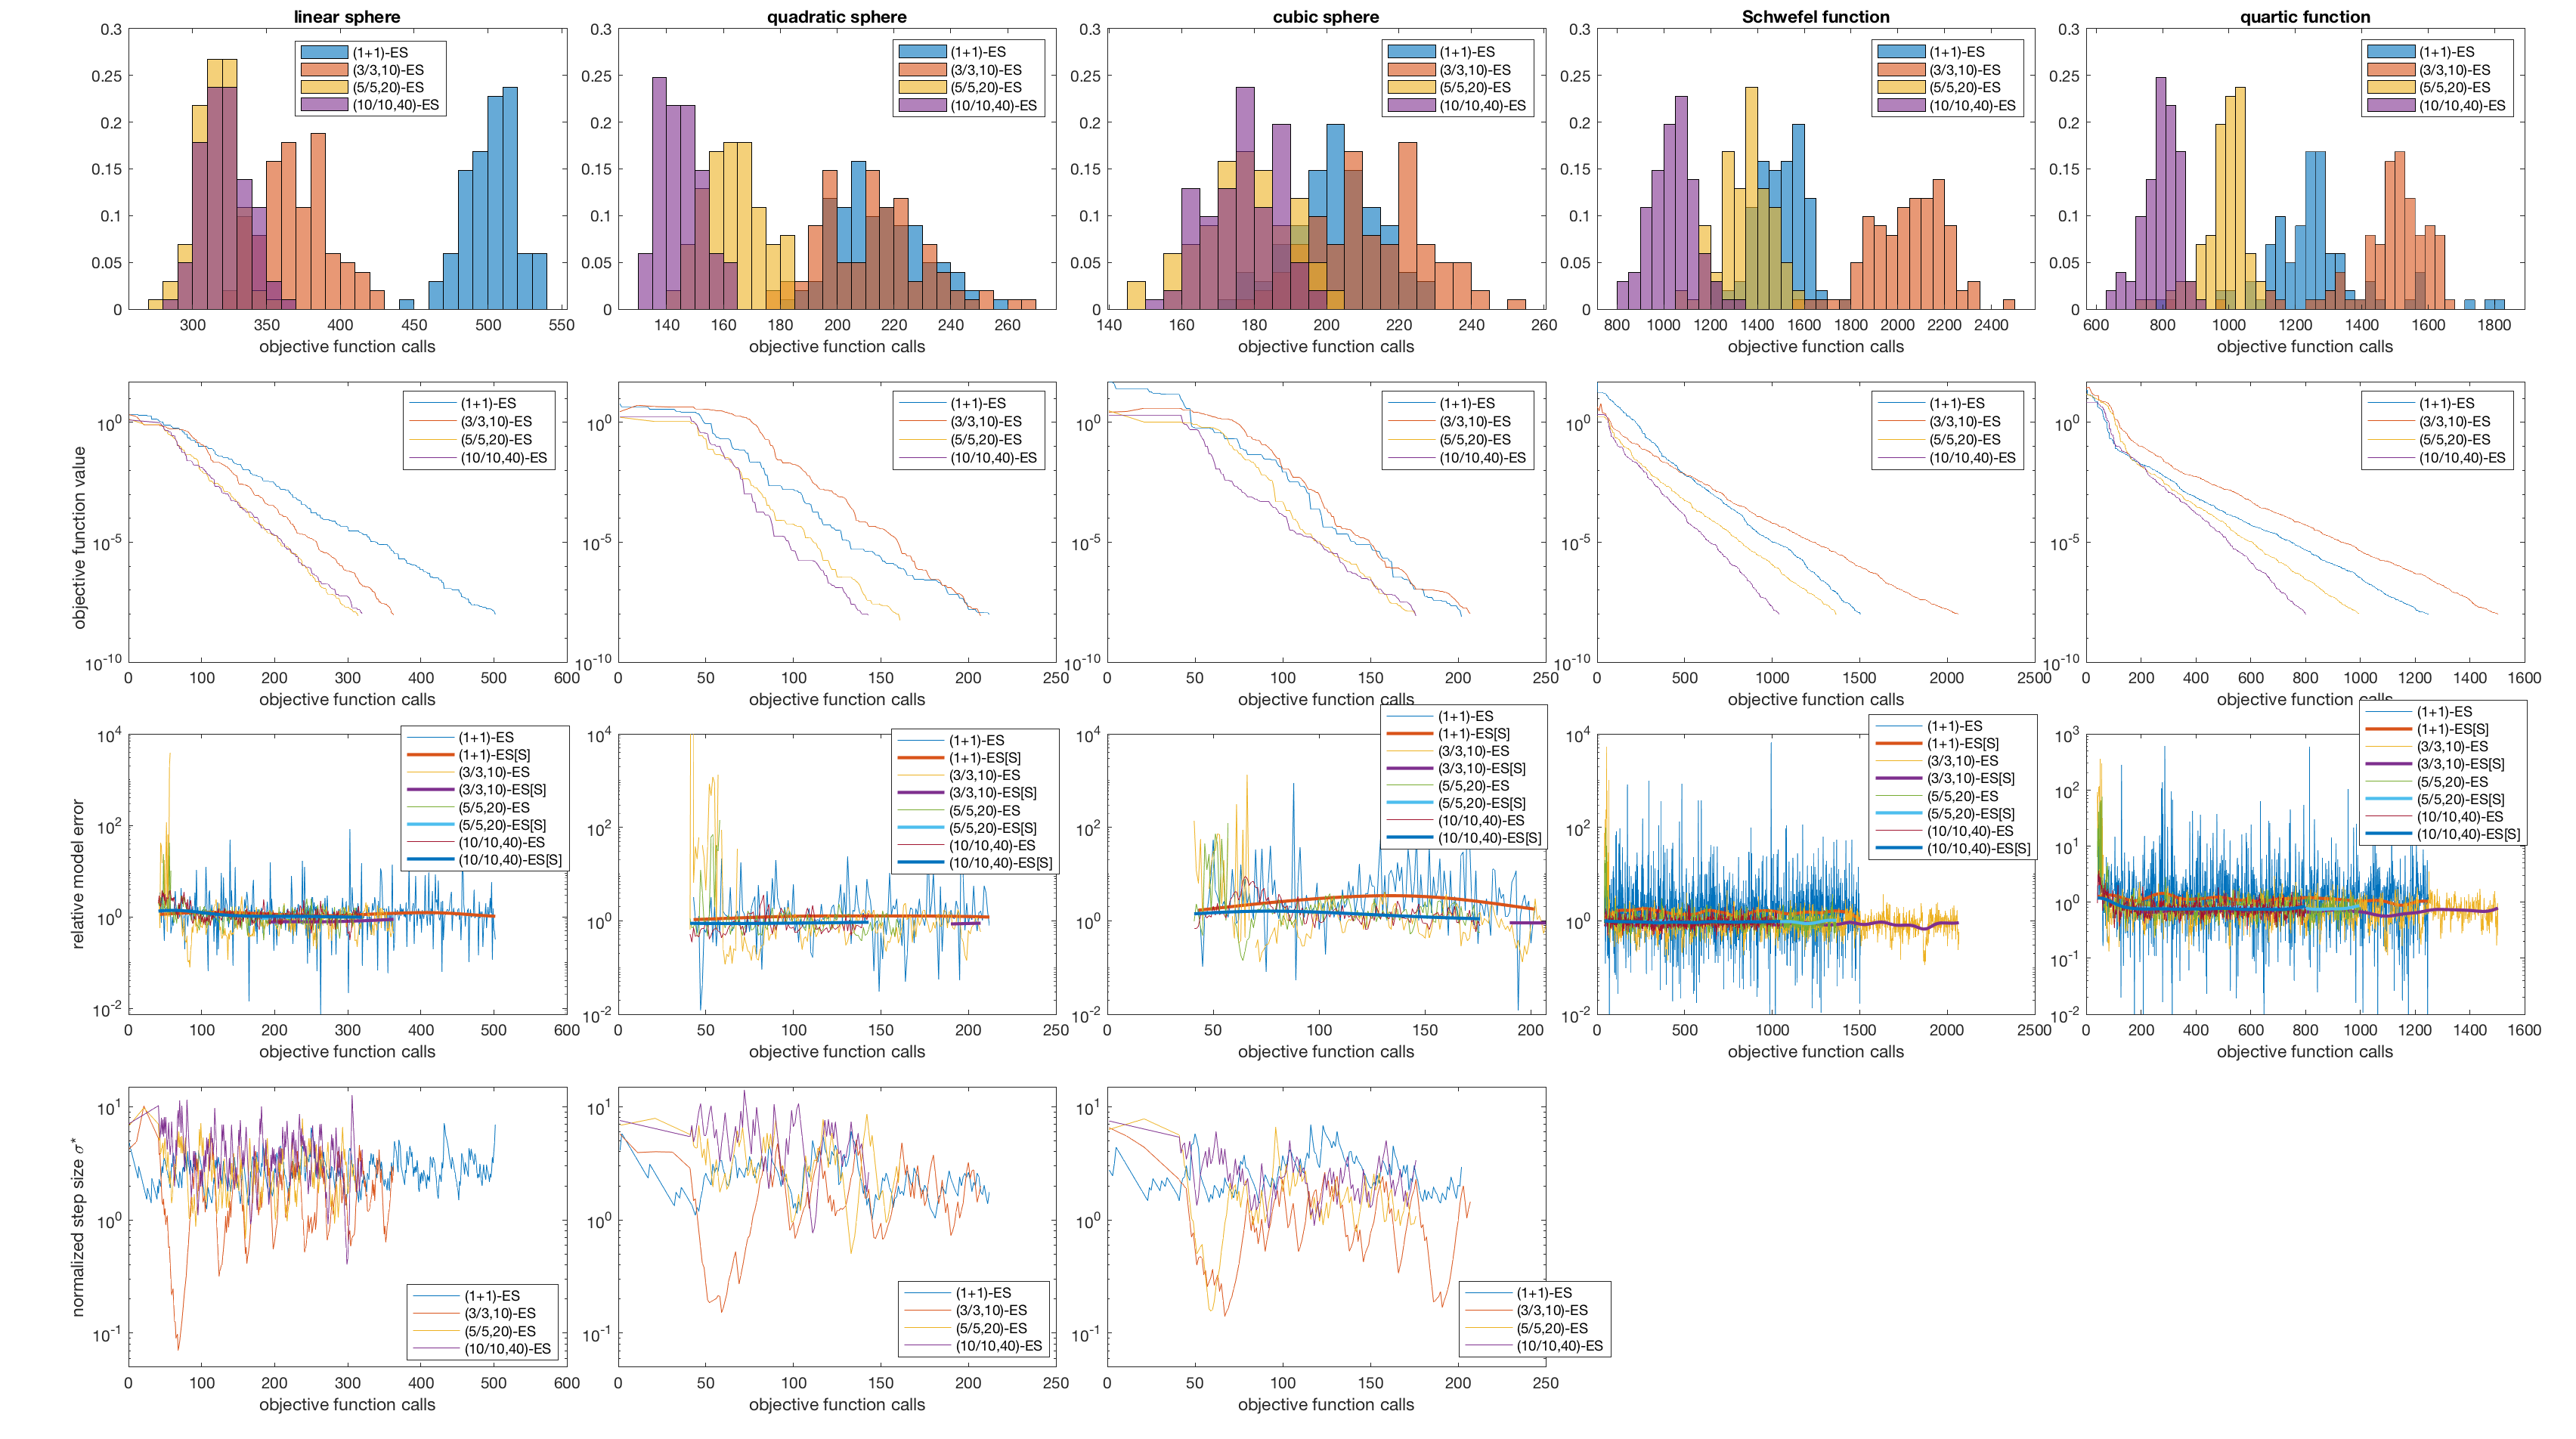
\includegraphics[height=4.3in, width=6.1in]{merged_plot_emergency_v4_final.pdf}
\caption{Results of GP-cross-ES obtained by applying the safeguard of plus-selection . Top row: Histogram showing the number of objective function calls needed to solve the five test problems. Second row: Convergence graphs observed in median runs. Third row: Relative model error obtained in median runs ([S] denotes the smoothed plot). Last row: normalized step size measured in median runs for sphere functions. }
\label{fig:merged_plot_GP-cross-ES}
\end{figure*}
\end{center}



To test the proposed GP-cross-ES and the step size adaptation mechanism, we use the same test functions and generate the corresponding Fig.s in Section 4.1. The number of objective function evaluations used in median runs and the corresponding speed-ups are reported in Table \ref{Tab:Test_result_GP-cross-ES}. The overall performance of GP-cross-ES improves as the population size increases, and outperforms the surrogate model assisted (1+1)-ES \cite{DBLP:conf/ppsn/KayhaniA18} in all test functions after $\lambda\geq 20$. The $\text{speed-up}_{\text{model}}$ for all three population sizes tested is around 1.5 for the linear sphere, between 1 and 1.5 for both the quadratic sphere and cubic sphere, about 0.7 to 1.4 for the Schwefel's function, and between 0.8 and 1.6 for the quartic function. The linear sphere does not seem to benefit much from a growing population size and the $\text{speed-up}_{\text{model}}$ seems to plateau after $\lambda \geq 20$; whereas in the quadratic sphere, Schwefel's function, and quartic function, the $\text{speed-up}_{\text{model}}$ does not show a clear sign of plateau. This observation also coincides with the $\text{speed-up}_{\text{self}}$ observed on the quadratic sphere, Schwefel's function, and quartic function where the growth in speed-up is proportional to the growth in population size. For example, in the Schwefel's function, the $\text{speed-up}_{\text{self}}$ doubles form 3.0 to 6.0 then approximately doubles to 12.7 after the population size doubles from 10 to 20 and finally 40. The histograms of objective function calls that are needed to solve each test problem (first row of Fig. \ref{fig:merged_plot_GP-cross-ES}) also illustrate the decrease in objective function calls needed to solve each test problem as the population size grows. Convergence graphs for the medium run are shown in the second row of Fig. \ref{fig:merged_plot_GP-cross-ES}. Linear convergence appears to be achieved in all runs. The third row reports the relative model error defined in Section 4.1. It is interesting that the relative model error for proposed GP-cross-ES (in any case of $\lambda$ being used) is still lower than that of the surrogate model assisted (1+1)-ES. One possible explanation for a larger variance in the relative model error observed for the surrogate model assisted (1+1)-ES (compared with the GP-$(\mu/\mu,\lambda)$-ES and GP-cross-ES) is the small population size (only a single offspring is generated), whereas the GP-$(\mu/\mu,\lambda)$-ES and GP-cross-ES generate $\lambda$ offspring in each generation. The bottom row in Fig. \ref{fig:merged_plot_GP-cross-ES} shows the normalized step size observed in median runs for the three sphere functions used. The normalized step size $\sigma^*$ in all runs are approximately between 0.5 and 10, where the strategy using plus-selection loses the benefit of a potential larger step size as opposed to the comma-selection (e.g., the $\sigma^*$ for the GP-$(\mu/\mu,\lambda)$-ES is significantly higher than that of the GP-cross-ES). Another observation is the decreasing trend in the variance of relative model error with a growing $\lambda$ for GP-cross-ES, which indicates the possibility of a potential good step resulting from using a large population size in selection and recombination. An illustration of the continuous occurrence of bad steps that can result in a continuous decrease of $\sigma^*$ is shown in the first 80 objective function calls in linear sphere for (3/3,10)-ES (GP-cross-ES with $\lambda=10,\mu=3$). But the occurrence or the length (the number of objective functions such situations take up) of such situations is reduced as $\lambda$ increases.


\begin{center}
\begin{figure*}
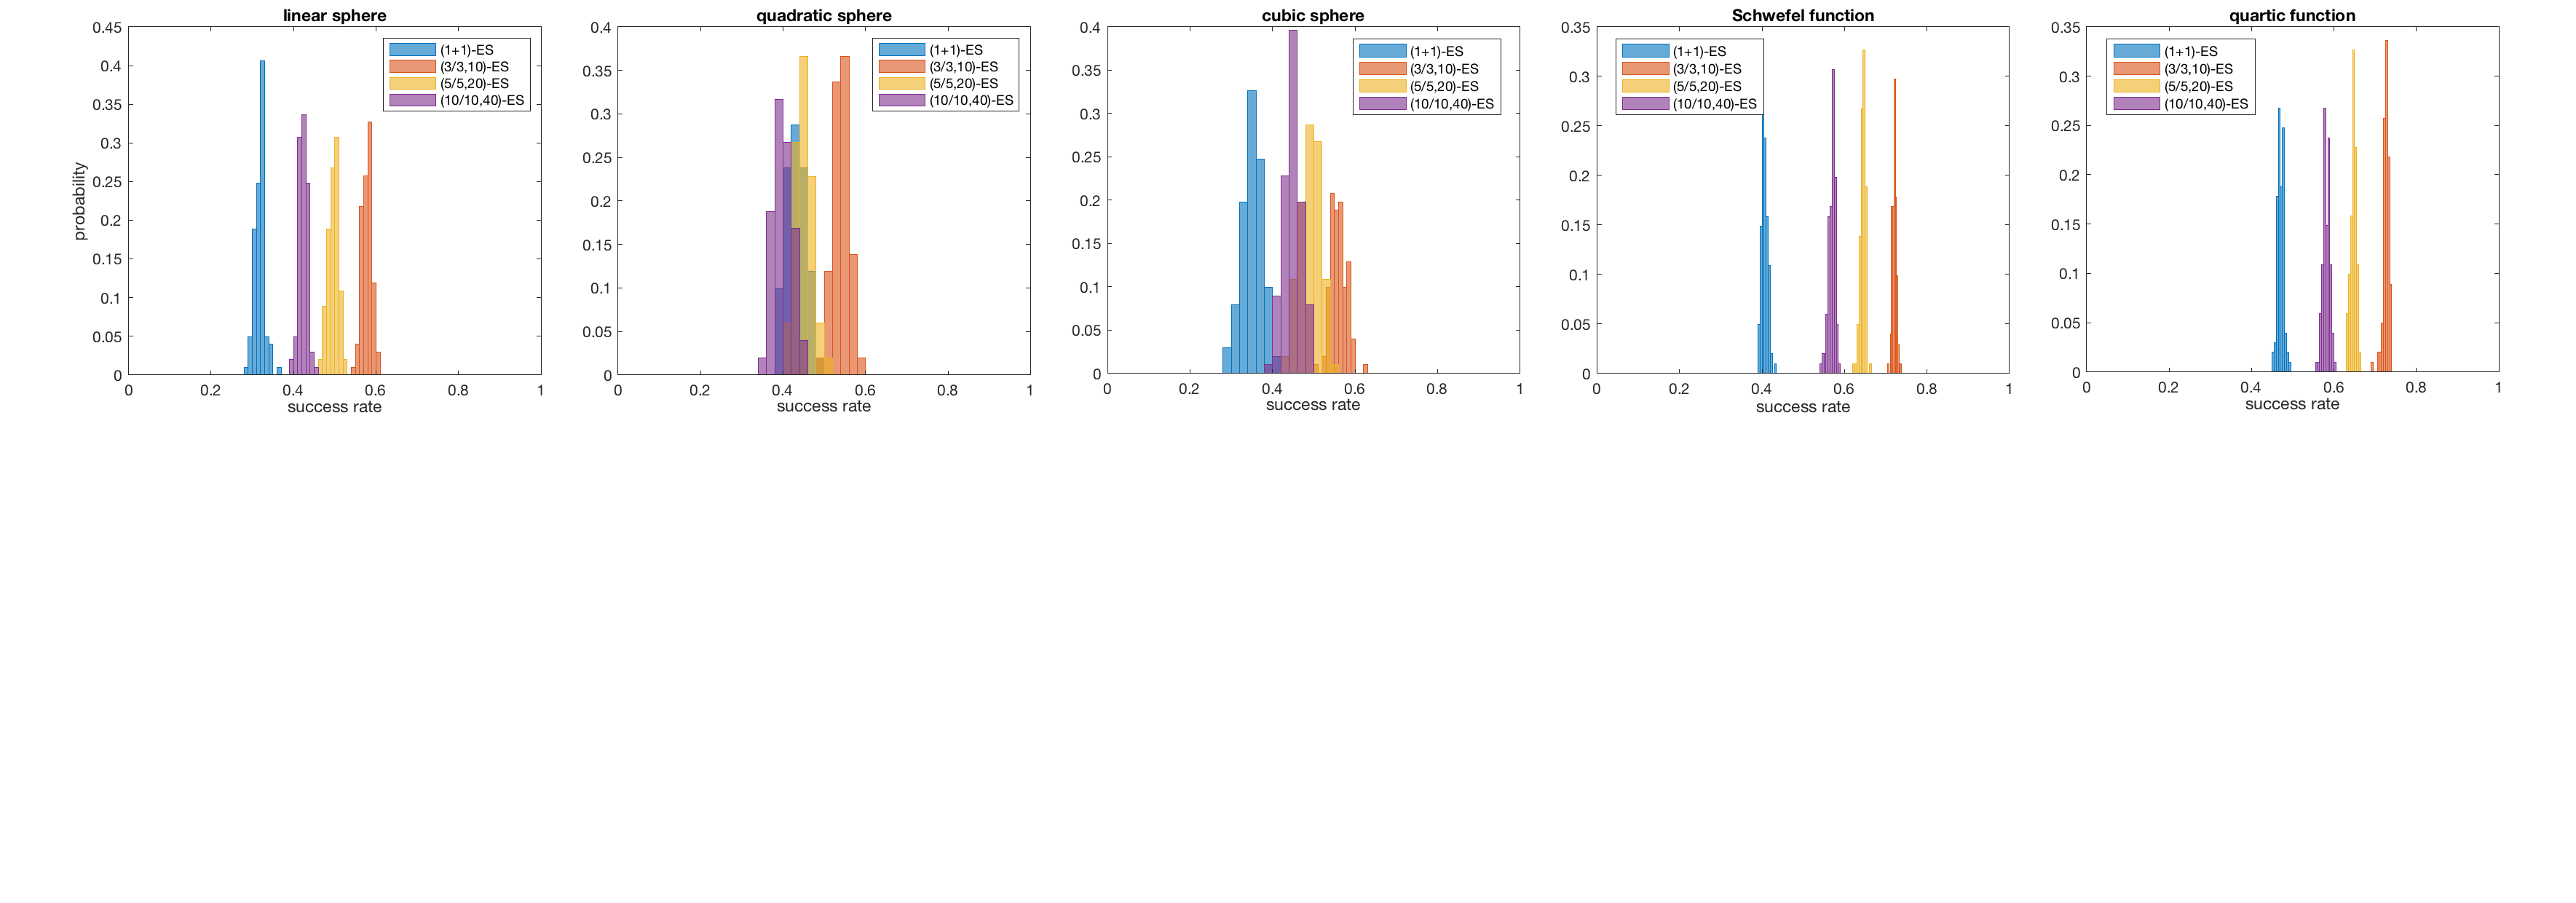
\includegraphics[height=1.2in, width=6in]{success_emergency_v3_final.pdf}
\caption{Result obtained by applying the safeguard of plus-selection. The first two rows show the normalized convergence rate for each run plotted in histogram and normalized probability density function (pdf) respectively. The last two rows represent the success rate (proportion of good step size in each run) plotted in histogram and pdf respectively. 
}
\label{fig:success_plot_GP-cross-ES}
\end{figure*}
\end{center}

%  is that the comma-selection can  
% The reduction in variance 

% of the model error for all tested strategies using plus-selection is much higher compared with the GP-mml-ES using comma-selection. 

% % Linear  that  is achieved for . The third row shows the relative model error for the median runs described in Section 4.1, it is interesting that the relative model error for surrogate assisted $(\mu/\mu,\lambda)$-ES with different population size is actually higher after the step size is adapted using the CSA with emergency, previous result in Section 3.1 shows (1+1)-ES with model assistance has higher relative model error, but the value is really close after using the new step size adaptation. The last row in Fig. \ref{fig:merged_plot_GP-cross-ES} shows the normalized step size, where the benefit of $(\mu/\mu,\lambda)$-ES is no longer obvious given the fact that we discard the inferior offspring, but it can be inferred that using a larger population size could reduce the variance in normalized step size.


% The first row in Fig. \ref{fig:merged_plot_GP-cross-ES} also illustrates the decrease of number of objective function calls needed to solve the test problems 

% For a population size of $40$, the speed up for sphere functions are 1.6, 1.5 and 1.2 for linear, quadratic and cubic respectively. It is notable that the speed-ups in linear sphere are between twice and three times before the emergency situation is proposed. For Schwefel' s function and quartic function, the strategy obtain a convergence rate of 0.35 and 0.5 respectively for a population size from 10 to 20 with 0.3 for both test functions for a population size from 20 to 40. 

% This is well illustrated in the histogram of objective function calls in first row of Fig. \ref{fig:merged_plot_GP-cross-ES} that the objective function calls for all functions reduces with a growing population size. 
% % $\color{red}{\text{will add more accurate data for comparison, including the range of GP error}}$    


Similarly, the histograms of success rates (the proportion of a good step size in each run) for all test problems are plotted in Fig. \ref{fig:success_plot_GP-cross-ES} by replicating 100 runs for each test problem. The success rate for GP-cross-ES is overall larger than that of the surrogate model assisted (1+1)-ES with the exception of the quadratic sphere in which the success rate of GP-cross-ES with $\lambda=10$ and $20$ being the same level as surrogate model assisted (1+1)-ES. For all other test functions, the success rate for GP-cross-ES decreases as $\lambda$ increases. In both the linear sphere and cubic sphere, the success rate for GP-cross-ES ranges from 0.4 to 0.5, 0.45 to 0.55, and 0.55 to 0.65 for $\lambda=10,20$, and $40$ respectively; whereas surrogate model assisted (1+1)-ES being about 0.3 to 0.35. The success rate observed in the Schwefel's function and quartic function are between 0.55 and 0.61; 0.62 and 0.65; and 0.70 and 0.75 for GP-cross-ES with $\lambda=10,20$, and $40$ respectively, and ranges from 0.55 to 0.62 for surrogate model assisted (1+1)-ES. Even if the success rate reduces with a lager $\lambda$ for GP-cross-ES, from the sharper slope, compared with GP-$(\mu/\mu,\lambda)$-ES, in the convergence plots, we can infer that the step is regarded as "good" by the GP-cross-ES has a potential better quality than that of GP-$(\mu/\mu,\lambda)$-ES. That is, the fitness gain obtained by taking the step is larger than that of the GP-$(\mu/\mu,\lambda)$-ES. By using a larger $\lambda$, the GP-cross-ES with proposed step-size adaption mechanism takes "good" steps that can bring potential larger fitness gain compared with the GP-$(\mu/\mu,\lambda)$-ES. One possible explanation of the better performance is the quality increase of taking the good steps outweighs the reduce in probability regarding the occurrence of a good step .  



% Histogram and probability density function of normalized convergence rate and success rate are plotted in Fig. \ref{fig:success_convergence_emergency}. The convergence rate for all population size grows significantly, almost doubled for all test functions despite a slight decrease in success rate (can also be interpreted as one minus the rate when emergency happens). It makes sense that the CSA with emergency rejects bad steps so that the quality of each step taken improves and therefore larger normalized convergence rate. Using CSA with emergency with a large population suggests an improvement in normalized convergence rate but a slight decrease in success rate for sphere functions. There is a trade-off between the two and finding the optimal relation can be a future goal to work on.


% $\color{red}{table(test\ functions)}$
% Table for median of test results for surrogate model assisted $(\mu/\mu,\lambda)$-ES using CSA with emergency



% Figure for success rate for surroagte assisted $(\mu/\mu,\lambda)$-ES with $\lambda = 10,20,40$





\section{Conclusions}
In this thesis, we applied the simple model of unbiased Gaussian distributed noise for surrogate modelling approach from Kayhani and Arnold \cite{DBLP:conf/ppsn/KayhaniA18} to analyze the surrogate model. By using this approach, we analyzed the behaviours of the proposed GP-$(\mu/\mu,\lambda)$-ES on the quadratic sphere function and observed a very significant $\text{speed-up}_{\text{self}}$ as the surrogate model is more fully exploited compared with the surrogate model assisted (1+1)-ES. If the surrogate model is accurate, we would expect a $\text{speed-up}_{\text{self}}$ equals to the population size $\lambda$. In experiments, the $\text{speed-up}_{\text{self}}$ achieved is about half the expected value for quadratic sphere and quartic function, a factor between two and six of the expected value for linear sphere and cubic sphere. In the Schwefel’ s function, the GP-$(\mu/\mu,\lambda)$-ES does not even converge when $\lambda \geq 20$. In most cases except in the quartic function, the performance of the GP-$(\mu/\mu,\lambda)$-ES is inferior to the surrogate model assisted $(1+1)$-ES. There is a factor approximately four between the analytical results and the experimental results for $\text{speed-up}_{\text{model}}$ in quadratic sphere function. One possibility is the assumption that the Gaussian noise are uncorrelated which may not hold in the case of generating multiple offspring in each iteration as is happened in $(\mu/\mu,\lambda)$-ES, but can be valid when generating a single offspring in (1+1)-ES. 

We tried to interpret the cause of the gap from the single step behaviour of the strategy. One observation is the increased success rate but a potential decreased quality of a good step compared with the surrogate model assisted (1+1)-ES, indicating many of the steps generated do not give much improvement (fitness gain). Based on the analysis and the observations of the GP-$(\mu/\mu,\lambda)$-ES, we proposed the GP-cross-ES and a corresponding step size adaptation mechanism taking benefit of the plus-selection where the bad steps are rejected. The strategy is evaluated numerically using a set of test functions. It shows that the step size adaptation mechanism adapted the step size successfully in all runs and the GP-cross-ES achieves an overall $\text{speed-up}_{\text{model}}$ about 1.4 to 1.6 for a population size $\lambda \geq 20$ in all five test functions. 



% We first replicated the analytical and experimental results obtained from the surrogate-model-assisted (1+1)-ES \cite{DBLP:conf/ppsn/KayhaniA18}. By doing the mentioned, we understood the use of this modelling approach (on Gaussian Process surrogate model) and testing ESs on simple test functions (specifically, quadratic sphere function) where the behaviours of the surrogate model and the strategy can be well interpreted. 


% Take the model from there, analyze the 

% found that using the simple model for surrogate model from K
% very significant speed-up observed, as the surrogate model assisted $(\mu/\mu,\lambda)$-ES more fully exploit the surrogate model. If the model is accurate, we would expect a speed-up of the population size $\lambda$. We then run experiements 

% many cases, performance inferiior to (1+1)-ES

% many of the step does not give improvements.

% Uncorrelated Gaussian noise is not 

% speed-up inferior to what have been hoped.

% Come up with the idea that plus-selection.

% primarily for those functions but not significant on the others.



In future work, we will study the behaviours of surrogate assisted CMA-ES using the same analysis that can potentially handle ill-conditioned problems. Further goals include length scale adaptation mechanism in the Gaussian Process and surrogate model accuracy control that can possibly further reduce the gap between the expected analytical results and the experimental results. 

\section*{Acknowledgment}
I would like to express my sincere gratitude my supervisor Dr. Dirk V. Arnold for his continuous support during the past two semesters, as well as his patience, motivation, and passion that motivates me all the time both in study and beyond. Besides my supervisor, I would like to thank my parents for their love and unconditional support during the past years without which I would not be where I am now. 

% For future work, we will work on a selection mechanism for candidate solutions deciding what candidate solutions to choose based on the fitness gain it may bring. Further, a step size adaptation mechanism for the surrogate model assisted (1 + 1)-ES should be considered. 


%\end{document}  % This is where a 'short' article might terminate




% \appendix
% %Appendix A
% \section{Headings in Appendices}
% The rules about hierarchical headings discussed above for
% the body of the article are different in the appendices.
% In the \textbf{appendix} environment, the command
% \textbf{section} is used to
% indicate the start of each Appendix, with alphabetic order
% designation (i.e., the first is A, the second B, etc.) and
% a title (if you include one).  So, if you need
% hierarchical structure
% \textit{within} an Appendix, start with \textbf{subsection} as the
% highest level. Here is an outline of the body of this
% document in Appendix-appropriate form:
% \subsection{Introduction}
% \subsection{The Body of the Paper}
% \subsubsection{Type Changes and  Special Characters}
% \subsubsection{Math Equations}
% \paragraph{Inline (In-text) Equations}
% \paragraph{Display Equations}
% \subsubsection{Citations}
% \subsubsection{Tables}
% \subsubsection{Figures}
% \subsubsection{Theorem-like Constructs}
% \subsubsection*{A Caveat for the \TeX\ Expert}
% \subsection{Conclusions}
% \subsection{References}
% Generated by bibtex from your \texttt{.bib} file.  Run latex,
% then bibtex, then latex twice (to resolve references)
% to create the \texttt{.bbl} file.  Insert that \texttt{.bbl}
% file into the \texttt{.tex} source file and comment out
% the command \texttt{{\char'134}thebibliography}.
% % This next section command marks the start of
% % Appendix B, and does not continue the present hierarchy
% \section{More Help for the Hardy}

% Of course, reading the source code is always useful.  The file
% \path{acmart.pdf} contains both the user guide and the commented
% code.

% \begin{acks}
%   The authors would like to thank Dr. Dirk V. Arnold for providing the
%   MATLAB code of the \textit{BEPS} method.

%   The authors would also like to thank the anonymous referees for
%   their valuable comments and helpful suggestions. The work is
%   supported by the \grantsponsor{GS501100001809}{National Natural
%     Science Foundation of
%     China}{http://dx.doi.org/10.13039/501100001809} under Grant
%   No.:~\grantnum{GS501100001809}{61273304}
%   and~\grantnum[http://www.nnsf.cn/youngscientists]{GS501100001809}{Young
%     Scientists' Support Program}.

% \end{acks}






\printbibliography

\end{document}
